%My thesis!
%\documentclass[11pt,a4paper,titlepage]{report}
\documentclass[a4paper,11pt,openright,twoside]{book}
\usepackage{amsmath}
\usepackage{ amssymb }
\usepackage{calligra}
\usepackage{amsfonts}
\usepackage[english]{babel}
\usepackage{verbatim}
\usepackage{indentfirst}
\usepackage{fancyhdr}
\usepackage{amsthm}
\usepackage{graphicx}
\usepackage{indentfirst}
\usepackage{microtype}
\usepackage{lmodern}
\usepackage{braket}
\usepackage{todonotes}
\usepackage{subcaption}

\usepackage[font=small,labelfont=bf]{caption}  %per la didascalia delle immagini
\usepackage{mathrsfs}  %per fare le lettere calligrafiche
\usepackage{bm}  %per mettere le lettere greche in grassetto
\usepackage[T1]{fontenc}     %pacchetto lettere accentate
\usepackage[utf8]{inputenc}   %pacchetto lettere accentate

\newtheorem*{remark}{Remark}

\newcommand{\HRule}{\rule{\linewidth}{0.5mm}}

% MER says: You can have no-indent later if you want to, but not while
% I'm reading this.
%\setlength\parindent{0pt} % toglie identazione ovunque
\usepackage[sc]{mathpazo}
\usepackage{tikz}

\newcommand{\mesh}{\mathcal{T}_t}

% -----------------

\begin{document}

%--------------------------

\begin{titlepage}
%\begin{adjustwidth*}{10pt}{-40pt}
\begin{center}
\vspace*{-2.7cm}

\includegraphics{images/aquila_nome}
\\
\rule{\textwidth}{1pt}
\\[0.5cm]
{\Large DEPARTMENT OF MATHEMATICS}
\\[0.35cm]
{\Large MASTER DEGREE IN MATHEMATICS}
\\[3.5cm]
\textsc{\huge \textbf{Simulating CSF flow in an idealized geometry of the subarachnoid space}}
%\\[0.4cm]
%{\Large March 25th, 2015}
%\\[3cm]
\\[4cm]
\begin{minipage}{0.5\textwidth}
\flushleft {
\large Advisors: \\
 \textbf{Prof. Eleuterio F. Toro} \rule{0pt}{2.5ex}\\
 \normalsize University of Trento\\[0.4cm]
\large \textbf{Dr. Marie E. Rognes} \\
\large \textbf{Ms. Eleonora Piersanti} \\
\large \textbf{Dr. Victor Haughton} \\
 \normalsize Simula Research Laboratory\\[0.4cm] \rule{0pt}{2.5ex}}\\
\end{minipage}
\begin{minipage}{0.45\textwidth}
\vspace{-3.2cm}
\flushright {\large
Student: \\
\rule{0pt}{2.5ex} \textbf{Carlo Cisale}\\
\normalsize University of Trento} \\
\end{minipage}

\vspace*{\fill}
{\textsc{\normalsize October $25^{th},$ $2017$}}
\rule{\textwidth}{1pt}


\end{center}
%\end{adjustwidth*}
\newpage
\thispagestyle{empty}
\phantom{}
\end{titlepage}
\newpage
\thispagestyle{empty}

\pagenumbering{roman}
\chapter*{\LARGE Acknowledgments}
There are many people I need to thank for this work. First of all, I want to thank Prof. Eleuterio F. Toro for being such a passionate instructor, who inspired me in going further and start this thesis. \\
I want to thank my supervisor Dr. Marie E. Rognes, who could always put me on the right path whenever I felt lost, or when something did not work. Thank you for giving me the opportunity to join Simula Research Laboratory, an experience that has taught me a lot, and that made me grow professionally and personally. \\
I thank Dr. Victor Haughton, for always being so optimistic and for having faith in math students like me. Collaborating with you has given me insights of mathematics that I have never thought of. \\

I would also like to thank Eleonora Piersanti, Vegard Vinje, Magne Nordaas, Øyvind Evju for their important help, and for always having the right answer to my questions. I feel very lucky to have had talented students like you around me, and I have certainly learned a lot thanks to you. \\

My stay in Norway  wouldn't have been the same without the Simula gang. I miss you guys all very much, and you made my six months in Oslo one of the best times of my life. \\
I thank all the beautiful people I met in Trento. All of you in different ways turned this city into my home, and I will never forget about it. \\
Last but not least, I thank my family for their constant support, for believing in me, and for making me the person I am now.

\newpage

%{\Large \textbf{List of acronyms}}



%--------------------------
\newpage
\tableofcontents


\newpage
\pagenumbering{arabic}

\chapter{Introduction}
% wiki
% article martin, kalata, loth,...
The field of computational fluid dynamics (or CFD) is helping medical doctors unveil mysteries of the human body, providing informations without the use of invasive procedures. For instance, nowadays it is possible to analyze a patients' blood flow in arteries or aneurysms, in order to get important informations on how to predict  aneurysms' rupture, or to study the effects of stenosis in arteries. The following study is an application of CFD to advance our understanding on Chiari I malformation.

The brain and the spinal cord are surrounded by the cerebrospinal fluid (CSF), a clear fluid that in an healthy person, is composed of dilute amounts of proteins and monoamines. It provides nutrients and remove waste from the brain, and acts as a cushion for the brain, providing damping between the brain and the skull when sudden movements of the cranium occur. The CSF moves in a pulsatile way through the subarachnoid space (SAS), a space between the arachnoid mater and the pia mater. The CSF flow is passive and its pulsatile nature has been associated with changes in blood volume within the cranial cavity due to the cardiac cycle \cite{silverthorn}.

More specifically, this thesis will focus on CSF flow in the domain of Chiari I malformation. Chiari I is a neurological disorder, where the bottom part of the brain, the cerebellum, descends out of the skull and crowds the spinal cord, putting pressure on both the brain and spine and causing many symptoms like severe headaches, balance problems, respiratory problems. Chiari symptoms are often complicated by related conditions like intracranial hypertension, tethered cord, or syringomyelia, a neurological condition where a fluid filled cyst, or syrinx, forms in the spinal cord. These syrinxes expand the spinal cord and stretch the nerve tissue paper thin. This could cause permanent nerve damage and paralysis [\emph{http://conquerchiari.org}].

Since advances in magnetic resonance imaging (MRI), the number of people affected by Chiari I malformation has increased. It is currently estimated that $1$ in $1000$ people have Chiari, which means $300000$ people in the United States alone. If left untreated, the progressing of the symptoms may have a lethal outcome [Stephany et al., 2008]. The only treatment which addresses the problem is surgery. Alternatively, some doctors monitor the situation and treat individual symptoms, but since surgery is the primary treatment option, most patients see a neurosurgeon for a better opinion. This surgical procedures is known as \textit{craniovertebral decompression}, which has the goal to create more room around the malformation and restore the flow of spinal fluid. During this procedure, typically a part of the skull is removed (\textit{craniectomy}), or parts of the vertebrae are removed (\textit{laminectomy}). After this first step, a \textit{duraplasty} is carried out, where the \textit{dura mater}, i.e. the covering of the brain, is opened and a patch is sewn in to make it bigger, increasing the movement of the tissue.
In the $40 \%$ of cases the surgical outcome is good, with no symptoms or limitations. In some other cases (around the $10-20 \%$), the procedure has poor improvements. 

In recent studies like \cite{sivarama}, medical doctors have studied the effect of compliance in the intracranial compartment, and concluded that an increase in the compliance is the most significant and consistent change measured after decompression surgery. 

The purpose of our study is to simulate CSF flow in an idealized geometry of the spinal cord. First, we assume that the walls of the spinal cord are rigid, to mimic the pre-operative case before the decompression surgery.  Afterwards, we introduce a prescribed movement on one of the boundaries, the tissue boundary, which will mimic the post-operative case and the increase in compliance of that portion of the spinal cord. This has been done solving Navier-Stokes equations using the finite element method library FEniCS for the simulations. Our final goal is to compare the different models and movements of the boundary, and study how changes in the fluid velocities, pressure, and stresses are affected by the compliance of the tissue. 

This thesis has the following outline. Chapter 2 yields an introduction to the medical background on the anatomy of the central nervous system, and on Chiari I malformation. Chapter 3 gives a description of the mathematical models that were used. In Chapter 4 we show the discretization of Navier-Stokes equations, and the numerical methods used to solve them. In Chapter 5 test cases on the verification of the N-S solvers are presented. Finally, in Chapter 6 and 7 we show the results of the simulations in an idealized geometry of subarachnoid space, and the conclusions on the study.

\chapter{Medical background}
In this chapter, a short description of medical background necessary to the understanding of the mathematical problem is presented. If not specified, the informations given below are based on the textbook ``\emph{Human Physiology}", by D.U. Silverthorn, and the \emph{Conquer Chiari} website, a <<non-profit organization dedicated to improving the experiences and outcomes of Chiari and syringomyelia patients through education, awareness, and research>>  (\emph{http://conquerchiari.org}).

\section{Anatomy of the Central Nervous System}
The human nervous system consists of the central nervous system (CNS), which includes the brain and the spinal cord, and the peripherical nervous system (PNS), which consists of sensory neurons.  The importance of CNS is due to the fact that it integrates informations that arrive from the sensory division of the PNS and determine whether a response is needed. 

\subsection{The Spinal Cord}
In vertebrates, the brain is encased in a bony skull, or cranium, and the spinal cord runs through a canal in the vertebral column. The body segmentation that is characteristic of many invertebrates is the bony \emph{vertebrae}, which are "piled up" on top of one another and separated by disks of connective tissue. 

\newpage

\begin{figure}[h!]
\centering
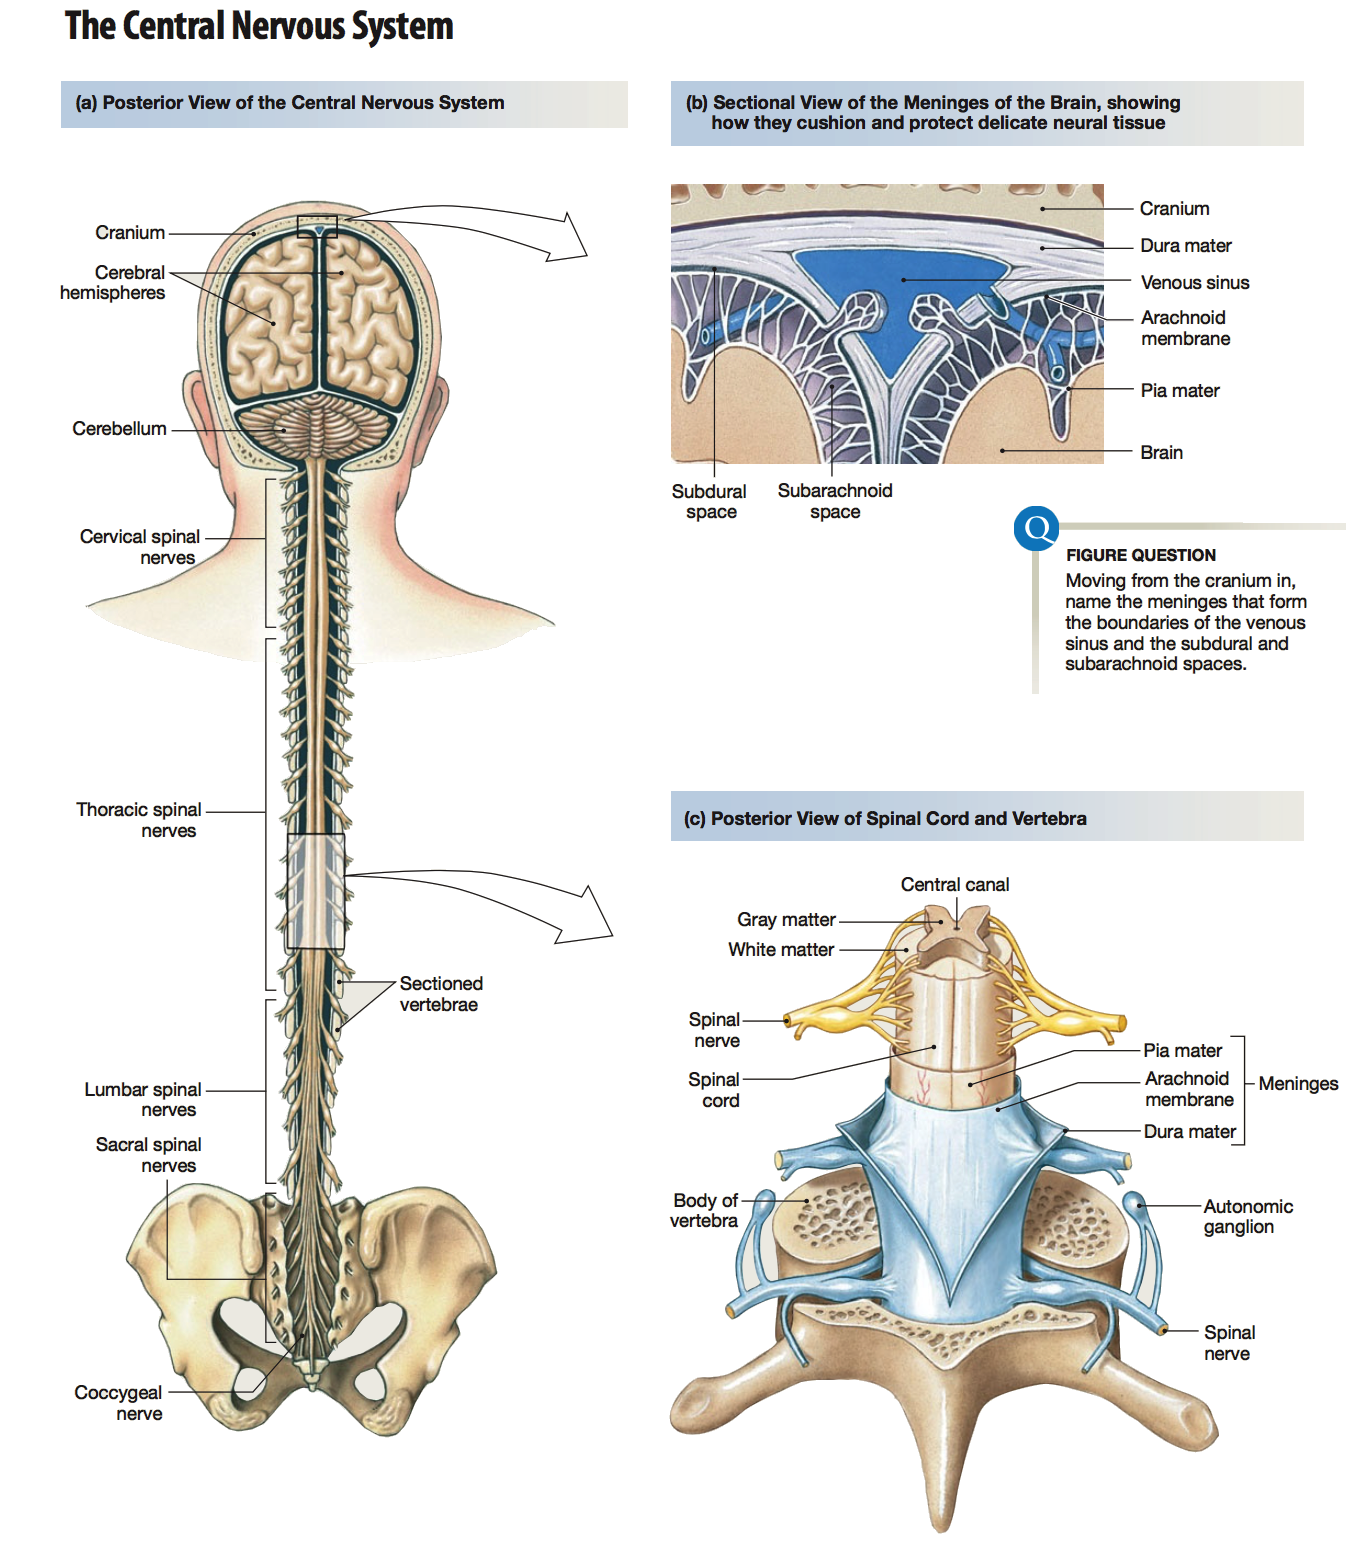
\includegraphics[width=\textwidth]{images/spinal_cord}
\label{img:cns:1}
\end{figure}

\newpage

The spinal cord is the major pathway for information flowing back and forth between the brain and the skin, joints, and muscles of the body. Moreover, in the spinal cord are present neural networks responsible for locomotion. It is divided into four regions (\emph{cervical, thoracic, lumbar} and \emph{sacral}), named to the corresponding adjacent vertebrae (see Fig. \ref{img:cns:1}). Each spinal region is subdivided into segments, and each segment gives rise to a bilateral pair of spinal nerves. Just before a spinal nerve joins the spinal cord, it divides into two branches called roots. Along the cord, there are 31 pairs of nerves: 8 in the cervical region, 12 in the thoracic region, 5 in the lumbar region, 5 in the sacral region. The first four segments of the cord are usually referred to as C1-C8, T1-T12, L1-L5, S1-S5 (Fig. \ref{img:cns:2}).

\begin{figure}[h!]
\centering
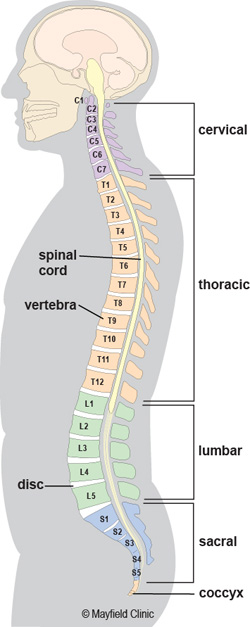
\includegraphics[width=.3\textwidth]{images/spine}
\caption{The segments of the spinal cord.}
\label{img:cns:2}
\end{figure}


The three layers covering the brain and the spinal cord are known as \emph{meninges}, that lie between the bones and tissue of the central nervous system. These membranes help stabilize the neural tissue and protect it from bruising against the bones. Starting from the bones towards the neural tissue, the membranes are the \emph{dura mater}, the \emph{arachnoid membrane}, and the \emph{pia mater}.

The \emph{cerebrospinal fluid}, or CSF, is a salty solution that is continuously secreted by a specialized region in the brain. From the brain, CSF flows into the \emph{subarachnoid space} (or SAS) between the pia mater and the arachnoid membrane, surrounding the entire brain and the spinal cord in fluid (see Fig. \ref{img:cns:3}). It provides nutrients and removes waste from the brain, and acts as a cushion for the brain, providing damping between the brain and the skull when sudden movements of the cranium occur.


\begin{figure}[h!]
\centering
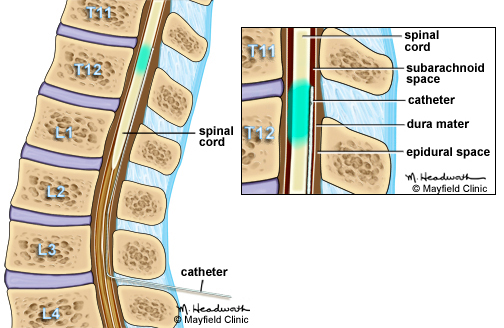
\includegraphics[width=.6\textwidth]{images/sas}
\caption{The SAS lies between the pia mater and the arachnoid membrane.}
\label{img:cns:3}
\end{figure}



\section{The Chiari I malformation}
Chiari I malformation is a neurological disorder where part of the brain, the cerebellum (or more specifically the cerebellar tonsils), descends out of the skull into the spinal area, obstructing the normal flow of the CSF. Chiari patients have a wide range of symptoms: severe headaches, pain in the neck, loos of motor control, respiratory problems, weakness. 

\begin{figure}[h!]
\centering
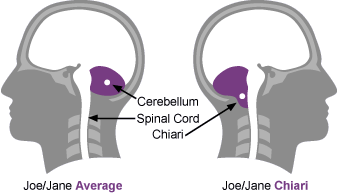
\includegraphics[width=.6\textwidth]{images/chiari}
\caption{Difference between an healthy patient (on the left) and a Chiari I patient (on the right) (\emph{http://conquerchiari.org}).}
\label{img:cns:4}
\end{figure}

In some cases, Chiari patients develop a neurological disorder known as \emph{syringomyelia}, where a fluid-filled cyst, a \emph{syrinx}, develops inside the spinal cord. This cyst can grow over time, causing the spinal cord to expand and stretch nerve tissue. Eventually, the syrinx can cause permanent nerve damage and paralysis. About $30\%-50\%$ of people with Chiari also have syringomyelia, but it can also form after a spinal cord injury, such as a car accident.

\begin{figure}[h!]
\centering
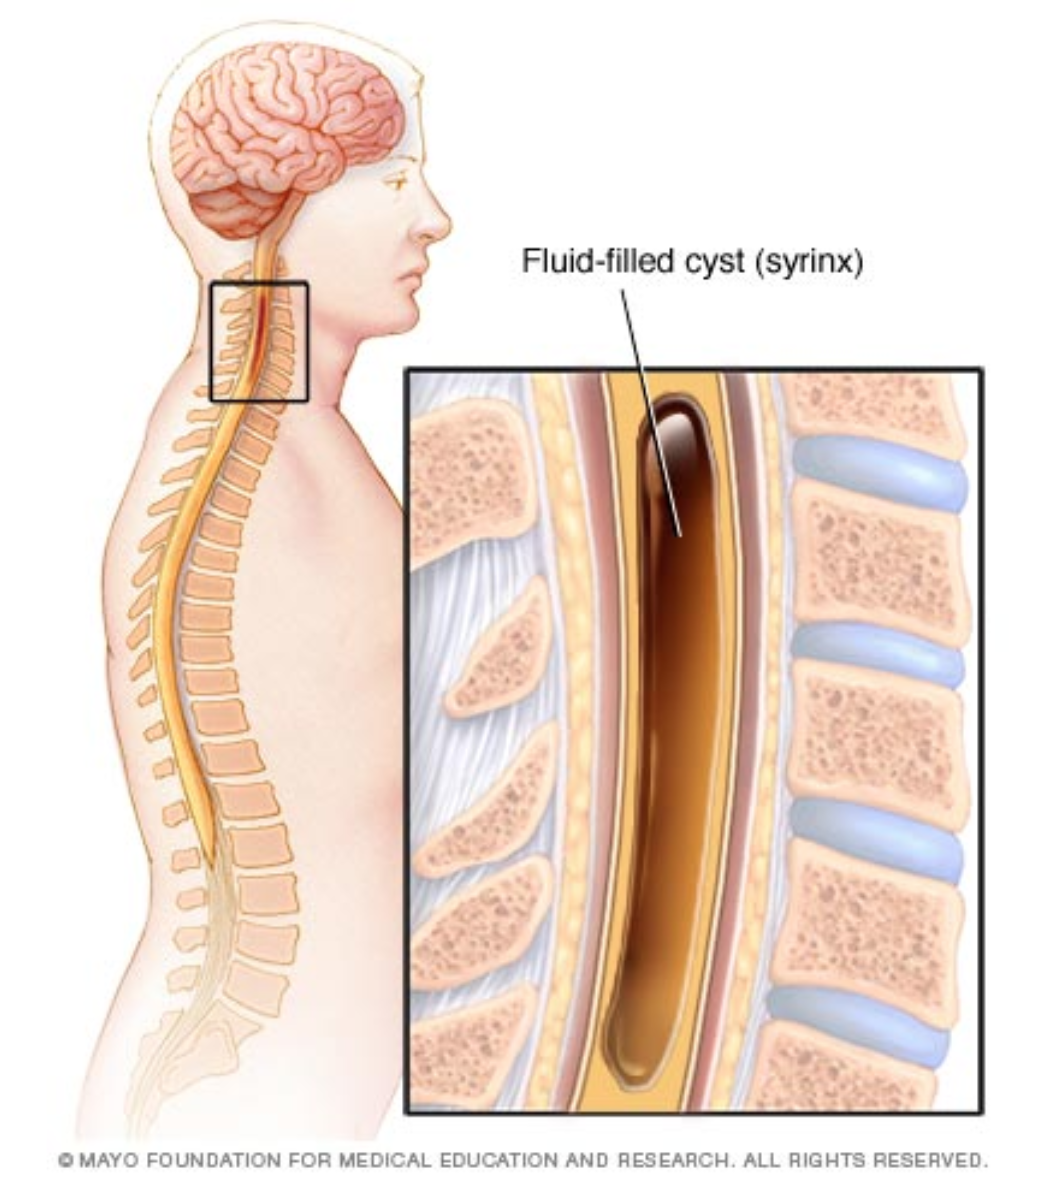
\includegraphics[width=.6\textwidth]{images/syrinx}
\caption{How a syrinx appears the spinal cord (\emph{http://www.mayoclinic.org}).}
\label{img:cns:5}
\end{figure}

Because of the risk of permanent nerve damage, if symptoms are significant and progressing, most surgeons with recommend a surgery known as \emph{craniovertebral decompression} or \emph{posterior fossa decompression} surgery. The goal of this operation is to create more room around the malformation and restore the flow of spinal fluid. 

Typically, during the procedure a part of the skull is removed (\textit{craniectomy}), or parts of the vertebrae are removed (\textit{laminectomy}). After this first step, a \textit{duraplasty} is carried out, where the dura mater is opened and a patch is sewn in to make it bigger, increasing the movement of the tissue.
In the $40 \%$ of cases the surgical outcome is good, with no symptoms or limitations. In some other cases (around the $10-20 \%$), the procedure has poor improvements. 



\chapter{Mathematical models}

\section{Derivation of the Navier-Stokes equations}
Navier-Stokes equations describe the motion of viscous fluid substances. They describe many phenomena, and may be used to model weather, water flow in pipes, air flow around a wing, and blood flow in arteries. In this section we give an overview on how these equations are derived. 

\subsection{Reynolds transport theorem}
The general conservation law from \cite{reynolds} states that any change in the quantity of any entity within a closed surface can only be affected in two different ways: it may be affected by the production or destruction of the entity within the surface, or by the passage of the entity across the surface. \\
The transport theorem can be approached in two ways. One is starting from a fixed set of spatial coordinates, a fixed \emph{control volume}, where fluid can enter and exit the boundaries of the defined body. The other is a control volume which consists of the same material particles at all times. Therefore, the body follows the flow, and no fluid will cross the boundary. In this approach, one has to take into account the movement of the boundary of the body, and the fact that body could change its volume. 

Let us consider a fixed control volume $\mathbf{V_0}$ and a fluid property $Q(\mathbf{x}, t)$, function of the position of the particle and time. The rate of change of $Q$ within the control volume can be written as

\begin{equation}
\frac{d}{dt} \int_{V_0} Q(\mathbf{x}, t) \, dV.
\end{equation}

The net change of $Q$ must be equal to the rate of change within the control volume plus the net rate of mass flow out of the volume. Hence,


\begin{equation}
\label{eq:rey:1}
\frac{d}{dt} \int_{V_0} Q(\mathbf{x}, t) \, dV = 
\int_{V_0} \frac{\partial Q(\mathbf{x}, t}{\partial t} \, dV +
\int_{S_0} Q(\mathbf{x}, t) \mathbf{v} \cdot \mathbf{n} \, dV
\end{equation}

where $\mathbf{u}$ denotes the fluid velocity, $\mathbf{n}$ is the outward pointing unit normal, and $S_0$ is the closed surface which bounds $V_0$. The previous equation is known as Reynolds transport theorem. The right hand side of (\ref{eq:rey:1}) can be rewritten using the divergence theorem on the last term, obtaining

\begin{equation}
\label{eq:rey:2}
\frac{d}{dt} \int_{V_0} Q(\mathbf{x}, t) \, dV = 
\int_{V_0} \Big[ \frac{\partial Q(\mathbf{x}, t) }{\partial t} + \nabla \cdot (Q(\mathbf{x}, t) \mathbf{\mathbf{u}})   \Big] \, d V.
\end{equation}

\subsection{The conservation of mass and momentum}
Let us set $Q(\mathbf{x}, t) = \rho(\mathbf{x}, t)$, where $\rho$ is the fluid density which we will denote simply with $\rho$. The conservation of mass the mass of the system must remain constant over time. This means

\begin{equation}
\label{eq:rey:3}
\frac{d}{dt} \int_{V_0} \rho  \, dV = 0.
\end{equation}

This equation can be rewritten using the transport theorem (\ref{eq:rey:2}):

\begin{equation}
\label{eq:rey:4}
\frac{d}{dt} \int_{V_0} \Big[ \frac{\partial \rho}{\partial t	} + \nabla \cdot (\rho \mathbf{u}) \Big] \, dV = 0.
\end{equation}

This equation holds for any volume $V_0$, hence the integrand has to be zero. Therefore, 

\begin{equation}
\label{eq:rey:5}
\frac{\partial \rho}{\partial t	} + \nabla \cdot (\rho \mathbf{u}) = 0.
\end{equation}

Equation (\ref{eq:rey:5}) is known as the \emph{continuity equation}. \\

In order to derive a similar equation for momentum, Newton's second law of motion is used. The net change of momentum must be equal to the applied forces which act on the system. The forces can be of two types: volume forces, acting on the entire control volume, and surface force, which act on the control volume surface. The forces acting on the forces are denoted by $\sigma_f \cdot \mathbf{n}$, where $\sigma_f = \sigma_f (\mathbf{u}, p)$ is the symmetric tensor denoting the total stress.

The balance of momentum requires that

\begin{equation}
\frac{d}{dt} \int_{V_0} \rho \mathbf{u} (\mathbf{x}, t) dV =
\int_{\partial V_0} \sigma_f \cdot \mathbf{n} dS + \int_{\partial V_0} \mathbf{F}_v dV,
\end{equation}

where $\mathbf{F}_v$ denote the volume forces. By applying the transport theorem to the left hand side, and the divergence theorem to the surface integral on the right hand side, we have

\begin{equation}
\frac{d}{dt} \int_{V_0} \Big[ \frac{\partial \rho \mathbf{u}}{\partial t} + \nabla \cdot (\rho \mathbf{v \cdot v}) - \nabla \cdot \sigma_f - \mathbf{F}_v \Big] dV = 0.
\end{equation}

As before, the integrand has to be zero. Rearranging we obtain 

\begin{equation}
\label{eq:rey:6}
\frac{\partial \rho \mathbf{u}}{\partial t} + \nabla \cdot (\rho \mathbf{u} \cdot \mathbf{u}) = 
\nabla \cdot \sigma_f + \mathbf{F}_v.
\end{equation}

If we assume that the density $\rho$ is constant, equation (\ref{eq:rey:6}) becomes

\begin{equation}
\label{eq:rey:7}
\rho \frac{\partial \mathbf{u}}{\partial t} + \rho \nabla \mathbf{u} \cdot \mathbf{u} - \nabla \cdot \sigma_f = \mathbf{F}_v.
\end{equation}

Equation (\ref{eq:rey:7}) is known as the \emph{momentum equation}.


\section{The Navier-Stokes equations on a fixed domain}

% References:
% - Quarteroni
% - Vegard
% - Drosdal

The flow in the SAS and in the spinal cord can be described by the incompressible Navier-Stokes equations for Newtonian fluids. In the future, we are going to assume that the density $\rho$ of the fluid is constant. The equations read

\begin{align}
\label{eq:ns:0}
\rho \dot{\mathbf{u}}
+ \rho \nabla \mathbf{u} \cdot \mathbf{u}
- \nabla \cdot \sigma(\mathbf{u},p)
&= \mathbf{f},  && \mathbf{x} \in \Omega, \, t>0 \\
\nabla \cdot \mathbf{u} &= 0, && \mathbf{x} \in \Omega, \, t>0
\end{align}

where $\Omega$ is our domain, and $\Omega \subset \mathbb{R}^2$.  We are going to solve the problem for the velocity field $\mathbf{u}(\mathbf{x},t)$, and the pressure field $p(\mathbf{x},t)$, where $\mathbf{x} = (x,y)$. The quantity $\sigma(\mathbf{u}, p)$, is the Cauchy stress tensor for a Newtonian fluid, given by

\begin{equation}
\sigma(\mathbf{u}, p) = \mu \nabla \mathbf{u} - p \mathbb{I}.
\end{equation}

The constant $\mu$ represents the fluid viscosity, while $\mathbf{f}$ denotes a forcing term per unit of mass. Substituting $\sigma$ in~\eqref{eq:ns:0} we obtain

\begin{align}
\rho \dot{\mathbf{u}} + \rho \nabla \mathbf{u} \cdot \mathbf{u} - \nabla \cdot (\mu \nabla \mathbf{u} - p \mathbb{I}) &= \mathbf{f}.
\end{align}

Since $\mu$ is constant, we have

\begin{align}
\label{eq:ns:3}
\rho \dot{\mathbf{u}} + \rho \nabla \mathbf{u} \cdot \mathbf{u} - \mu \Delta \mathbf{u} +  \nabla p &= \mathbf{f}, \\
\label{eq:ns:3bis}
\nabla \cdot \mathbf{u} &= 0.
\end{align}

The term $(\mathbf{u} \cdot \nabla)\mathbf{u}$ describes the process of convective transport \cite{quarteroni1}.\\
In order for the problem to be well posed, it is necessary to assign an initial condition

\begin{equation}
\mathbf{u} (\mathbf{x}, 0) = \mathbf{u}_0(\mathbf{x}) \quad \forall \mathbf{x} \in \Omega,
\end{equation}

where $\mathbf{u}_0$ is a given divergence-free vector field, together with suitable boundary conditions, such as

\begin{align}
\mathbf{u}(\mathbf{x},t) &= \phi (\mathbf{x}, t) & \forall \mathbf{x} \in \Gamma_D \\
\label{eq:ns:8}
\left( \mu \frac{\partial \mathbf{u}}{\partial \mathbf{n}} - p\mathbf{n} \right) (\mathbf{x},t) &= \psi(\mathbf{x},t) & \forall \mathbf{x} \in \Gamma_N
\end{align}


where $\phi$ and $\psi$ are given vector functions, while $\Gamma_D$ and $\Gamma_N$ give a partition of the domain boundary $\partial \Omega$, that is $\Gamma_D 	\cup \Gamma_N = \partial \Omega, \mathring{\Gamma}_D \cap \mathring{\Gamma}_N = \emptyset$. Moreover, $\mathbf{n}$ is the outward unit normal vector to $\partial \Omega$. Equation (\ref{eq:ns:8}) can also be written in another form

\begin{equation}
\sigma \cdot \mathbf{n} = \psi(\mathbf{x}, t)  \quad \forall \mathbf{x} \in \Gamma_N.
\end{equation}

\begin{remark}
\normalfont{In our notation, if $\mathbf{u} = (u_x, u_y)^T$ and $\mathbf{x} = (x, y)^T$, then $\nabla \mathbf{u}$ is defined as

\[
\nabla \mathbf{u} =
\begin{pmatrix}
\frac{\partial u_x}{\partial x} & \frac{\partial u_x}{\partial y} \\
\frac{\partial u_y}{\partial x} & \frac{\partial u_y}{\partial y}
\end{pmatrix}
\]


}
\end{remark}


\section{Navier-Stokes on a moving domain}
% From Donea, Duarte, Vegard

Numerical simulation of two-dimensional viscous incompressible fluid with free boundaries is getting a lot of attention in the past decades for the several applications in industry and medicine. An important consideration when coding problems in this class is the use of an appropriate \emph{kinematical description} of the continuum. Such a choice determines the relationship between the deforming continuum and the finite mesh of the computing zones, and the ability of the numerical method to deal with large distortions. \\
The algorithm of continuum mechanics usually make use of two classical descriptions of motion: the \emph{Lagrangian} description and the \emph{Eulerian} description. The arbitrary Lagrangian-Eulerian description (or ALE) has the advantage to combine the classical kinematical descriptions, while reducing their drawbacks. \\
In Lagrangian algorithms, each individual node of the computational mesh follows the associated material particle during motion, and they are mostly used in structural mechanics.
In Eulerian algorithms the computational mesh is fixed and the continuum moves with the respect to the grid. These algorithms are widely used in fluid dynamics problems.
In order to combine the best features of both algorithms, the ALE description was developed. We are going to talk about it later. Now let us focus on the classical descriptions of motion. \\
If not specified, the informations given below are based on Donea et al. \cite{donea}, Doarte et al. \cite{duarte}, and Vinje V. \cite{vegard}. 


\subsection{Lagrangian and Eulerian descriptions of motion}
Let us consider a domain $\Omega_{\mathbf{X}} \in \mathbb{R}^3$ consisting of material particles $\mathbf{X}$. The domain can undergo deformations, and the deformed domain $\Omega_\mathbf{x}$ is the current configuration at time $t$.

\begin{figure}[h!]
\centering
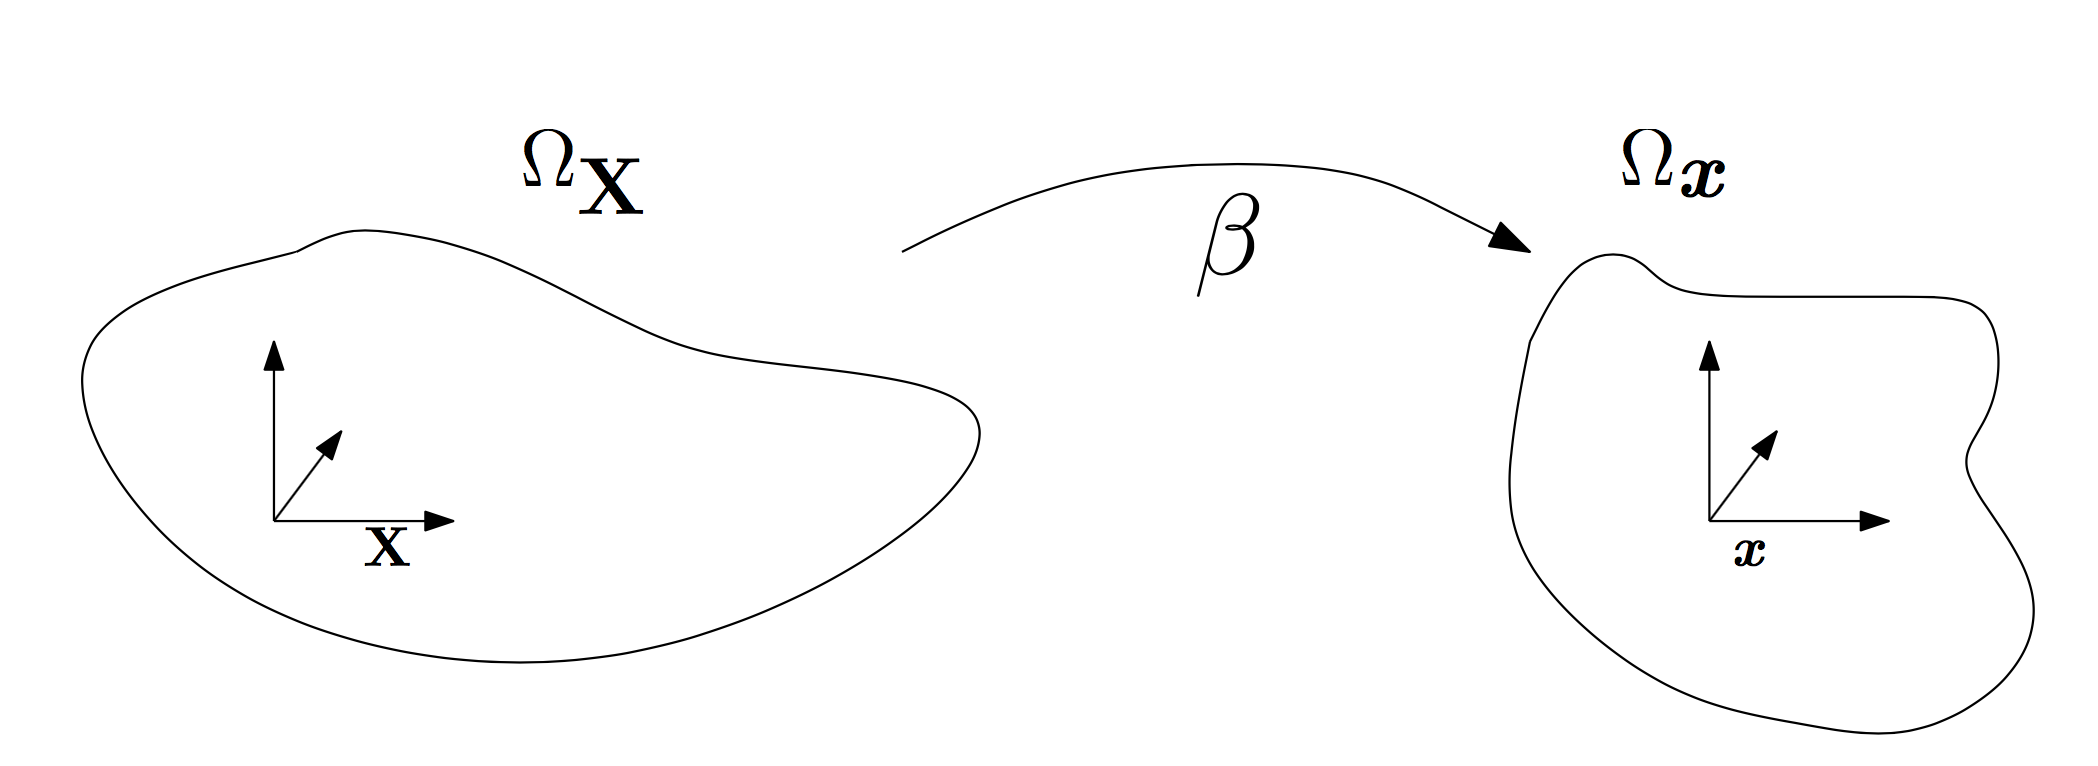
\includegraphics[width=\textwidth]{images/ALE1}
\caption{Lagrangian description of motion. The mapping $\beta$ maps the reference coordinates into the spatial ones.}
\end{figure}

We define one-to-one mapping:

\begin{align*}
\beta : \Omega_{\mathbf{X}} \times [0, T]  \rightarrow \Omega_\mathbf{x} \times [0, T] \\
(\mathbf{X} , t)  \rightarrow \beta(\mathbf{X}, t) = (\mathbf{x}, t),
\end{align*}

which takes any point $\mathbf{X}$ in the reference configuration to a new position $\mathbf{x} = \beta(\mathbf{X},t)$ at time $t$. As the mapping is one-to-one, it is also possible to keep track of the history of the motion by the inverse $\beta^{-1}$. Time is measured with the same variable $t$ in both domains. The gradient of $\beta$ with respect to $(\mathbf{X},t)$ can be written in the matrix forms as

\begin{equation}
\frac{\partial \beta}{\partial(\mathbf{X}, t)} = 
\begin{pmatrix}
\frac{\partial \mathbf{x}}{\partial \mathbf{X}} & \mathbf{u} \\
\mathbf{0}^T & 1
\end{pmatrix}
\end{equation}

where the material velocity

\begin{equation}
\mathbf{u}(\mathbf{X}, t) = \frac{\partial \mathbf{x}}{\partial t} {\Big |}_\mathbf{x},
\end{equation}

is the temporal change in the spatial variable $\mathbf{x}$ while holding $\mathbf{X}$ fixed, while $\mathbf{0}^T$ denotes a null vector. \\
In the Lagrangian description all the quantities are expressed in terms of the reference configuration $\Omega_{\mathbf{X}}$ and time, i.e. even though the material is deformed, we can still compute displacements and particle velocities using the material coordinates $\mathbf{X}$.
Since the grid coincides with the material coordinates, there are no convective term in the Lagrangian description, and it coincides with a moving control volume consisting of the same material points at all time. When a material undergoes large deformations, or for instance vortices or turbulences occur, the material velocity becomes difficult to handle in the Lagrangian approach.

In fluid mechanics, the \emph{Eulerian} approach describes the flow of a fluid through a fixed region in space and in each point we can measures its properties and quantities, such as velocity, pressure, temperature. The conservation equations in the Eulerian description are expressed in terms of the spatial coordinates $\mathbf{x}$ and time, and are neither connected to a reference configuration nor the material coordinates. Hence, large deformations are not an issue, since the material can enter and leave the fixed domain. The movement of a material through a fixed region results in convective effects, and convective operators can often be problematic in computational fluid dynamics since they are not symmetric.


\subsection{The Arbitrary-Eulerian Lagrangian formulation}
The ALE formulation is common is fluid-structure interaction problems and it provides a referential system which is neither attached to the material points nor totally fixed in space, i.e. the nodes of the computational mesh may be moved with the continuum in normal Lagrangian fashion, or be held fixed in Eulerian manner, or be moved in some arbitrarily specified way.

The following derivation is taken from [Donea, Vegard].

Since we need a new set of coordinates, an independent referential system with reference coordinates $\chi$ is introduced. Hence, we have two new mappings to relate all the configurations as shown in the picture below.

\begin{figure}[h!]
\centering
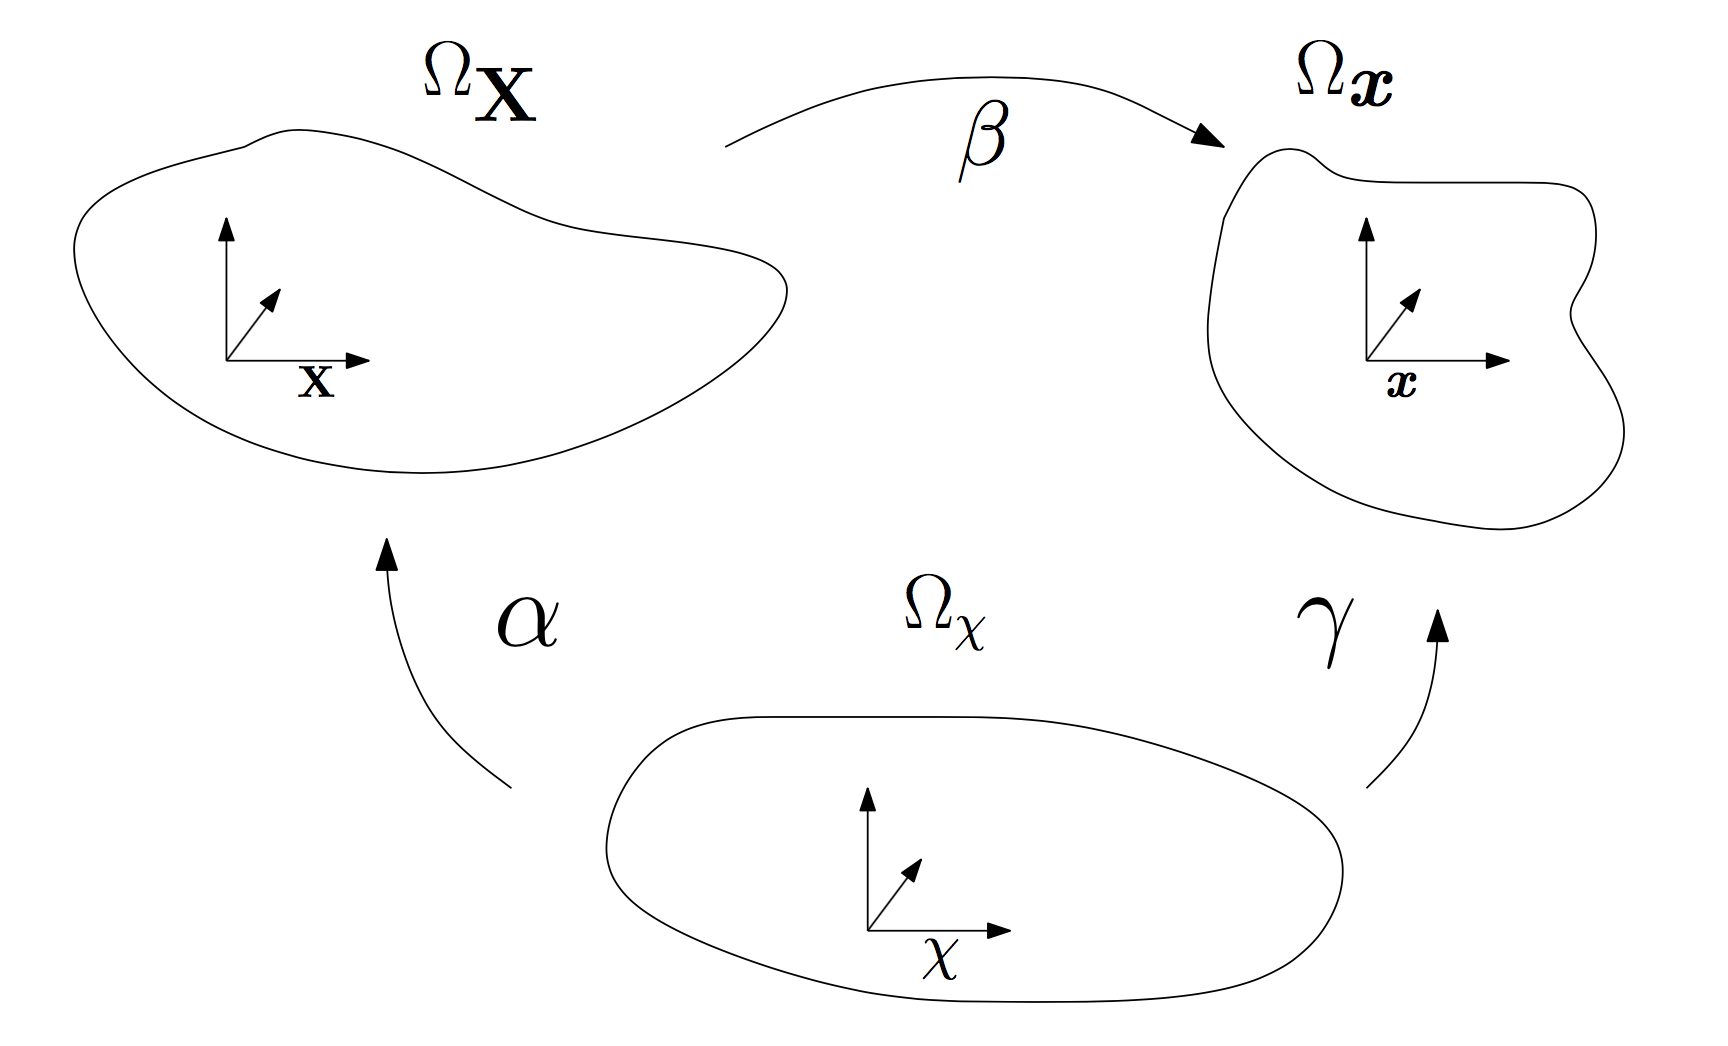
\includegraphics[width=\textwidth]{images/ALE2}
\caption{The three domains needed in the ALE formulation.}
\end{figure}

The mappings are defined similarly to $\beta$:

\begin{align*}
\gamma : \Omega_{\chi} \times [0, T]  \rightarrow \Omega_\mathbf{x} \times [0, T] \\
(\chi , t)  \rightarrow \gamma(\chi, t) = (\mathbf{x}, t),
\end{align*}


and the gradient of $\gamma$ is 

\begin{equation}
\frac{\partial \gamma}{\partial(\chi, t)} = 
\begin{pmatrix}
\frac{\partial \mathbf{x}}{\partial \chi} & \mathbf{w} \\
\mathbf{0}^T & 1
\end{pmatrix}
\end{equation}

where we define $\mathbf{w}$ as the mesh velocity, i.e.

\begin{equation}
\mathbf{w}(\chi, t) = \frac{\partial \mathbf{X}}{\partial t} {\Big |}_\chi,
\end{equation}

Hence, the fluid moves with velocity $\mathbf{u}$ and the domain moves with velocity $\mathbf{w}$.

To complete the relation between the different velocities, we define the inverse of $\alpha$ as

\begin{align*}
\alpha^{-1} : \Omega_{\mathbf{X}} \times [0, T]  \rightarrow \Omega_\chi \times [0, T] \\
(\mathbf{X} , t)  \rightarrow \alpha^{-1}(\mathbf{X}, t) = (\chi, t),
\end{align*}


Its gradient is given by

\begin{equation}
\frac{\partial \alpha^{-1}}{\partial(\mathbf{X}, t)} = 
\begin{pmatrix}
\frac{\partial \chi}{\partial \mathbf{X}} & \hat{\mathbf{u}}\\
\mathbf{0}^T & 1
\end{pmatrix}
\end{equation}

where the velocity

\begin{equation}
\label{eq:ale:4}
\hat{\mathbf{u}} (\mathbf{X},t) = \frac{\partial \chi}{\partial t} {\Big |}_{\mathbf{X}}
\end{equation}

denotes the temporal change in the reference system while keeping the material particle $\mathbf{X}$ fixed. Therefore, the velocity $\mathbf{\hat{v}}$ can be interpreted as the particle velocity in the referential domain.

Since $\beta = \gamma \circ \alpha^{-1} = \gamma(\alpha^{-1}(\mathbf{X},t))$ and obtain a relation between the different velocities by differentiating $\beta$:

\begin{align*}
\frac{\partial \beta}{\partial (\mathbf{X},t)} (\mathbf{X},t)
& = \frac{\gamma}{\partial (\chi, t)}(\alpha^{-1}(\mathbf{X},t)) \frac{\partial \alpha^{-1}}{\partial(\mathbf{X},t)}(\mathbf{X},t) \\
& = \frac{\partial \gamma}{\partial (\chi, t)}(\chi,t)) \frac{\partial \alpha^{-1}}{\partial(\mathbf{X},t)}(\mathbf{X},t).
\end{align*}

In matrix form, the previous equation reads

\begin{equation}
\begin{pmatrix}
\frac{\partial \mathbf{x}}{\partial \mathbf{X}} & \mathbf{u}\\
\mathbf{0}^T & 1
\end{pmatrix} = 
\begin{pmatrix}
\frac{\partial \mathbf{x}}{\partial \chi} & \mathbf{w}\\
\mathbf{0}^T & 1
\end{pmatrix}
\begin{pmatrix}
\frac{\partial \chi}{\partial \mathbf{X}} & \hat{\mathbf{u}}\\
\mathbf{0}^T & 1
\end{pmatrix}
\end{equation}

Multiplying the matrices on the right hand side, we obtain the following equation

\begin{equation}
\mathbf{u} = \frac{\partial \mathbf{x}}{\partial \chi} \cdot \hat{\mathbf{u}} + \mathbf{w}
\end{equation}

that relates the different velocities. We define the \emph{convective velocity} as

\begin{equation}
\mathbf{c} := \mathbf{u} -\mathbf{w} = \frac{\partial \mathbf{x}}{\partial \chi} \cdot \hat{\mathbf{u}}
\end{equation}

which is the relative velocity between the material and the mesh.

In order to obtain relations between quantities to formulate the balance equations, let us define the scalar quantity $Q$ defines as $Q^{*}(\mathbf{x},t)$, $Q(\chi,t)$, and $Q^{**}(\mathbf{X},t)$ in the spatial, reference, and material domain respectively.
To obtain a relation between the spatial description $Q$, and the material description $Q^{**}$ we use the previous the mapping $\beta$ that we have previously used:

\begin{equation}
Q^{**}(\mathbf{X},t) = Q(\beta(\mathbf{X},t),t) = Q \circ \beta.
\end{equation}

The gradient of $Q^{**}$ can then be computed as

\begin{equation}
\label{eq:ale:1}
\frac{\partial Q^{**}}{\partial (\mathbf{X}, t)} (\mathbf{X},t) = 
\frac{\partial Q}{\partial (\mathbf{x}, t)} (\mathbf{x},t)
\frac{\partial \beta}{\partial (\mathbf{X}, t)} (\mathbf{X},t),
\end{equation}

or in the matrix form

\begin{equation}
\label{eq:ale:2}
\begin{pmatrix}
\frac{\partial Q^{**}}{\partial \mathbf{X}} & \frac{\partial Q^{**}}{\partial t}
\end{pmatrix} = 
\begin{pmatrix}
\frac{\partial Q}{\partial \mathbf{x}} & \frac{\partial Q}{\partial t}
\end{pmatrix}
\begin{pmatrix}
\frac{\partial \mathbf{x}}{\partial \mathbf{X}} & \mathbf{u}\\
\mathbf{0}^T & 1
\end{pmatrix} 
\end{equation}

Multiplying the matrices, we obtain the equation that relates material and spatial derivatives:

\begin{equation}
\label{eq:ale:3}
\frac{\partial Q^{**}}{\partial t} = \frac{\partial Q}{\partial t}
+ \frac{\partial Q}{\partial \mathbf{x}} \cdot \mathbf{u}
\end{equation}

To ease notation we now recognize the material and spatial time derivatives $\frac{\partial Q^{**}}{\partial t} = \frac{\partial Q}{\partial t} {\Big |}_\mathbf{X}, \,  \frac{\partial Q}{\partial t} = \frac{\partial Q}{\partial t} {\Big |}_\mathbf{x}$, and define the material and spatial derivatives in the following way

\begin{equation}
\frac{d}{dt} := 	\frac{\partial}{\partial t} {\Big |}_\mathbf{X} \qquad
\frac{\partial}{\partial t} := \frac{\partial}{\partial t} {\Big |}_\mathbf{x}
\end{equation}

Now we can rewrite the relation (\ref{eq:ale:3}) can be written in the form

\begin{equation}
\label{eq:ale:6}
\frac{d Q}{d t} = \frac{\partial Q}{\partial t} + (\mathbf{u} \cdot \nabla) Q.
\end{equation}

The next step is to relate the material and the reference description, respectively $Q^{**} and Q^{*}$, by the mapping $\alpha$. This relation is the following

\begin{equation}
Q^{**} = Q^{*} \circ \alpha^{-1}.
\end{equation}

By proceeding as in (\ref{eq:ale:1})-(\ref{eq:ale:2}), we obtain the relation between material and reference time derivatives:

\begin{equation}
\label{eq:ale:3}
\frac{\partial Q^{**}}{\partial t} = \frac{\partial Q^{*}}{\partial t}
+ \frac{\partial Q}{\partial \chi} \cdot \hat{\mathbf{u}}.
\end{equation}

To express the spatial derivative of $Q^{*}$ in the spatial domain, we use the definition of $\hat{\mathbf{u}}$ from equation (\ref{eq:ale:4}) and obtain

\begin{equation}
\frac{\partial Q^{**}}{\partial t} = \frac{\partial Q^{*}}{\partial t}
+ \frac{\partial Q}{\partial \mathbf{x}} \cdot \mathbf{c}.
\end{equation}

This equation can be rewritten in the more common notation

\begin{equation}
\label{eq:ale:5}
\frac{d Q}{d t} = \frac{\partial Q}{\partial t} {\Big |}_\chi + (\mathbf{c} \cdot \nabla) Q
\end{equation}

and it is called the \emph{fundamental ALE equation}, which states that the time derivative in the material configuration is equal to its local (reference) derivative plus a convective term, taking into account the relative difference in velocity between the two systems. These relations also hold for vector quantities.

By combining equations (\ref{eq:ale:5})-(\ref{eq:ale:6}) we have

\begin{equation}
\label{eq:ale:7}
\frac{\partial Q}{\partial t} = \frac{\partial Q}{\partial t} {\Big |}_\chi - (\mathbf{w} \cdot \nabla) Q.
\end{equation}

which relates the spatial time derivative to the reference time derivative.


To write appropriate balance equations in the ALE framework we start by the balance equations written in terms of the material derivatives

\begin{align}
\frac{d \rho}{d t} &= \frac{\partial \rho}{\partial t} + \mathbf{u} \cdot \nabla \rho = - \rho \cdot \nabla \mathbf{u}, \\
\rho \frac{d \mathbf{u}}{d t} &= \rho (\frac{\partial \mathbf{u}}{\partial t} + (\mathbf{u} \cdot \nabla)\mathbf{u}) = \nabla \cdot \sigma
\end{align}

Using equation (\ref{eq:ale:7}), the spatial time derivatives can be replaced to obtain its ALE formulation

\begin{align}
\frac{\partial \rho}{\partial t} {\Big |}_\chi + \mathbf{c} \cdot \nabla \rho = - \rho \nabla \cdot \mathbf{u}, \\
\rho (\frac{\partial \mathbf{u}}{\partial t} {\Big |}_\chi + (\mathbf{c} \cdot \nabla)\mathbf{u}) = \nabla \cdot \sigma. 
\end{align}

The previous equations hold in \emph{any} time-dependent domain which does not necessarily coincide with the movement of material particles. The latter also shows that in order to obtain the ALE formulation from the Eulerian formulation is to replace the convective velocity with the relative velocity between the material and the mesh.

\newpage

\section{Modelling the idealized geometry of the SAS}



The simulations carried out in this thesis imitate the CSF flow through a region $\Omega \subset \mathbb{R}^2$ throughout time $t \in [0, T]$, where $T=15$ is the final time (and the number of cardiac cycles of our simulations, that we need in order for the flow to fully develop). Since cerebrospinal fluid consists of $99 \% $ of water \cite{linge1}, it can modeled as water at $37^{\circ} C$ [Hentschel et al., 2010]. The region surrounding the fluid is modelled as impermeable.
In the first section, we will use Navier-Stokes equation in a fixed domain to simulate the case with no movement of the boundary, while in the second one we will use the ALE formulation of Navier-Stokes equations and allow one of the boundaries to move in order to mimic the post-operative case where the tissue is more compliant. The table below describes the units and values used for the different parameters.

\begin{table}[h!]
\begin{center}
\begin{tabular}{| c | c | c | c |}
\hline
\textbf{Symbol} & \textbf{Meaning} & \textbf{Unit} & \textbf{Chosen value} \\
\hline
$\mathbf{u}$ & fluid velocity & $\frac{cm}{s}$ & to be computed \\
\hline
$p$ & pressure & $Pa$ & to be computed \\
\hline
$\rho$ & density & $\frac{kg}{cm^3}$ & $10^{-3}$ \\
\hline
$\mu$ & fluid viscosity & $\frac{cm^2}{s}$ & $0.700 \cdot 10^{-2 \, [\rm a] \, }$ \\
\hline
\end{tabular}
\end{center}
\caption{Variables and parameters of our models. See (Linge et. al. 2011) for $[a]$.}
\end{table}




\subsection{Fixed boundary}
Let us consider a two-dimensional rectangular (fixed) domain $\Omega^0 = [0, 4]
\times [0, 40]$, representing the right portion of the subarachnoid space, between the spinal cord and the dura mater from C1 to C5 vertebrae, approximately. We define the
\begin{itemize}
\item
  top boundary: $\partial \Omega_{\rm top}^0 = \{ (x, y) | y = 40\}$;
\item
  bottom boundary: $\partial \Omega_{\rm bottom}^0 = \{ (x, y) | y = 0\}$;
\item
  tissue boundary: $\partial \Omega_{\rm tissue}^0 = \{ (x, y) | x = 4\}$;
\item
  cord boundary: $\partial \Omega_{\rm cord}^0 = \{ (x, y) | x = 0\}$;
\end{itemize}
and thus $\partial \Omega^0 = \partial \Omega_{\rm top}^0 \cup
\partial \Omega_{\rm bottom}^0 \cup \partial \Omega_{\rm cord}^0 \cup
\partial \Omega_{\rm tissue}^0$.



\begin{figure}[h!]
\begin{minipage}[b]{.5\textwidth}
\centering
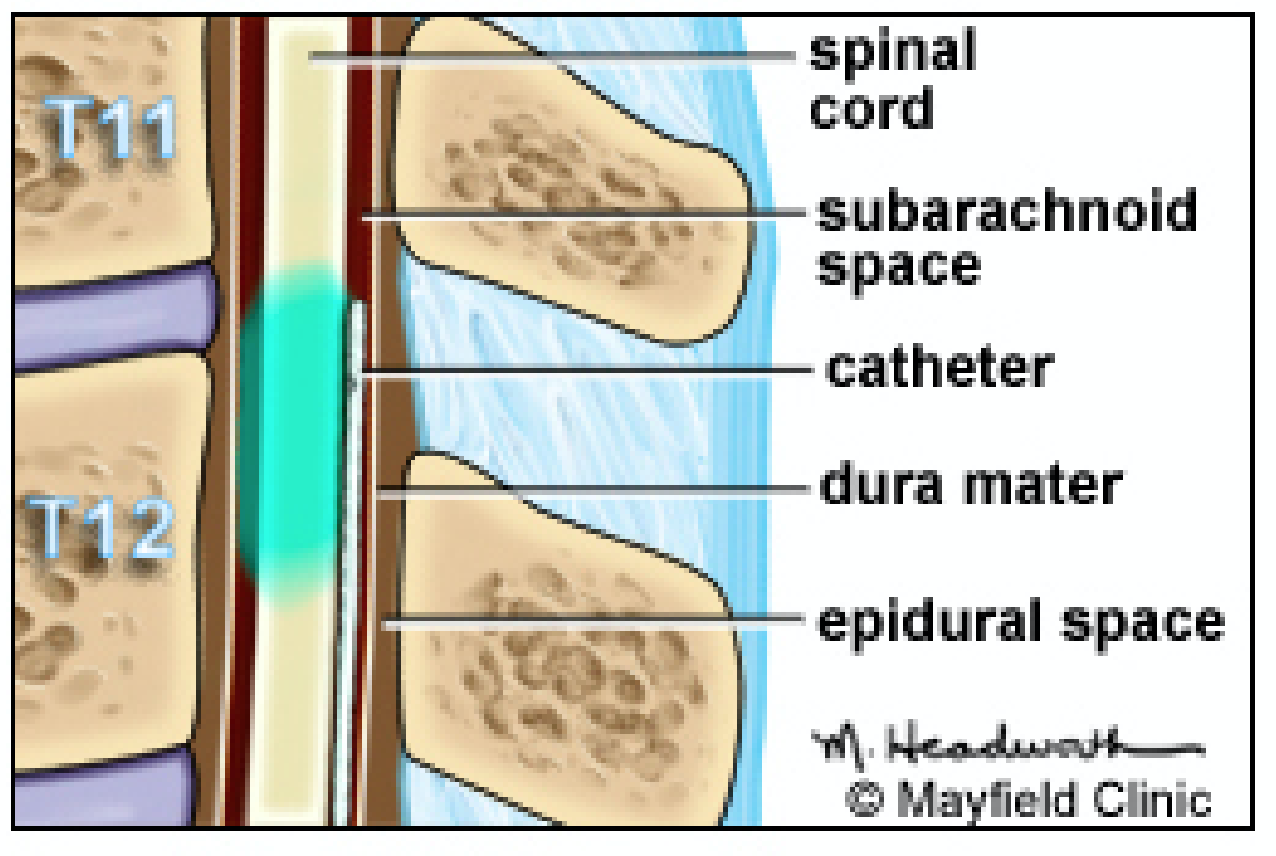
\includegraphics[width=.9\textwidth]{images/sas2}
\caption{Spinal cord in the SAS.}
\label{img:cns:3}
\end{minipage}
\begin{minipage}[b]{.4\textwidth}
\centering
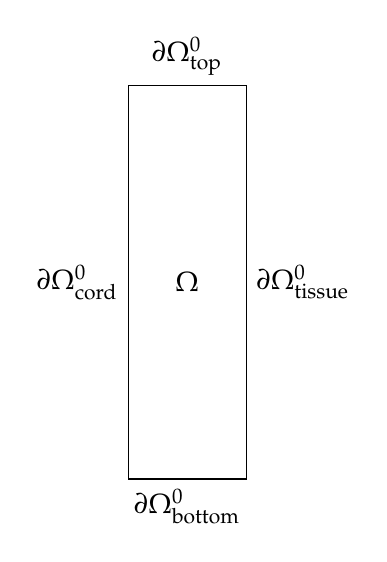
\begin{tikzpicture}
\node[
      draw,
      minimum height=5cm,
      minimum width=1.5cm,
      label=0:$\partial \Omega^0_{\rm tissue}$,%< -- This uses angle zero degree on the border for the location
      label=west:$\partial \Omega^0_{\rm cord}$, %< -- This uses an anchor of the node for the location
      label=north:$\partial \Omega^0_{\rm top}$,
      label=south:$\partial \Omega^0_{\rm bottom}$
] at (0,1.5) {$\Omega$};
\end{tikzpicture}
\caption{Schematic illustration of computational domain.}
\label{img:cns:4}
\end{minipage}
\end{figure}


We set the following boundary condition on $\partial \Omega^0$: on the boundaries $\partial \Omega_{\rm cord}^0$ and $\partial \Omega_{\rm tissue}^0$ we set the so called \emph{no-slip condition} $\mathbf{u = 0}$, i.e. the fluid velocity on those boundaries is zero. This condition does not allow the fluid to flow through the boundaries.
In order to simulate an oscillatory fluid flow, we set a pressure difference on the top and bottom boundaries, as follows:

\begin{align}
\label{eq:bc:6}
\sigma \cdot \mathbf{n} &= \mu \frac{\partial \mathbf{u}}{\partial \mathbf{n}} - p \mathbf{n} = -\bar{p} \mathbf{n} && \text { on } \partial \Omega_{\rm top}^0 \\
\label{eq:bc:6bis}
\sigma \cdot \mathbf{n} &= \mu \frac{\partial \mathbf{u}}{\partial \mathbf{n}} - p \mathbf{n} = \mathbf{0}  && \text { on } \partial \Omega_{\rm bottom}^0.
\end{align}

where $\bar{p}(t) = A \cdot sin(2\pi t)$ is a prescribed pressure, and $A = 4kPa$. We assume a heart rate of $60$ heart-beats per minute, so that the duration of the cardiac cycle is set to $1s$. During \textit{systole}, as blood flows into the brain, CSF flows down the Aqueduct of Sylvius. During \textit{diastole}, the opposite occurs. The sine term is added to reproduce the pulsatile motion of the fluid. 

\begin{figure}[h!]
\centering
\begin{tikzpicture}
\node[
      draw,
      minimum height=5cm,
      minimum width=1.5cm,
      label=0:$\mathbf{u = 0}$,%< -- This uses angle zero degree on the border for the location
      label=west:$\mathbf{u = 0}$, %< -- This uses an anchor of the node for the location
      label=north:$\sigma \cdot \mathbf{n} \equiv - \bar{p} \, \mathbf{n}$,
      label=south:$\sigma \cdot \mathbf{n} \equiv \mathbf{0} $
] at (0,1.5) {$\Omega$};
\end{tikzpicture}
\caption{Boundary conditions on the spinal cord for both fixed and moving domain.}
\label{img:cns:4}
\end{figure}

%\caption{Boundary conditions applied on $\partial \Omega^0$}

\newpage


\subsection{Moving boundary}
Our next step is to allow the domain and its boundary to move, and
solve the Navier-Stokes equations on this deforming domain. Let $\Omega^t$ denote the fluid domain which depends on time $t$, and
$\Omega^0$ denote the fixed fluid domain at $t = 0$. In
fluid-structure interaction, the fluid domain $\Omega^t$ consists of
the same material particles at all times, and moves with the material
points within the structure. Also assume that we have a mesh $\mesh$
of the domain $\Omega^t$. Let $\mathbf{w}$ denote the \emph{mesh velocity}.
  
%and $\mathbf{y}$ the \emph{mesh displacement} with respect to the reference domain $\Omega^0$, and thus by definition $\dot{\mathbf{y}} = \mathbf{w}$ where the superposed dot denotes the time derivative. 

%The movement of the domain $\Omega^t$ is governed by the mesh
%displacement, i.e.~for all $x(t) \in \Omega^t$, each corresponding to
%a point $\mathbf{X}_0 \in \Omega^0$, we have that
%\begin{equation}
%  \mathbf{X}(t) = \mathbf{X}_0 + \mathbf{y}(t)(X_0).
%\end{equation}
%\todo[inline]{Check the precise formulation carefully in Donea
%  reference e.g.}

An ALE formulation of the Navier-Stokes equations on the deforming
domain $\Omega^t$ reads: find the velocity $\mathbf{u}$ and the
pressure $p$ such that
\begin{align}
  \label{eq:ns:1}
  \rho \dot{\mathbf{u}}
  + \rho \nabla \mathbf{u} \cdot (\mathbf{u} - \mathbf{w})
  - \mu \Delta \mathbf{u} + \nabla p
  &= \mathbf{f},  & \text{in } \Omega^t, \\
  \label{eq:ns:2}
  \nabla \cdot \mathbf{u} &= 0, & \text{in } \Omega^t,
\end{align}
for $t \in (0, T]$. The quantity $\mathbf{f}$ is a given body force.
We will let the fluid domain boundary follow the changes on the
fluid-structure interface. Moreover, to move the entire domain, we
will use a \emph{Laplacian smoothing}
algorithm [Winslow, 1963]. More precisely, our mesh smoothing
equation reads: given some boundary velocity $\mathbf{w}_0$, find
$\mathbf{w}$ that satisfies
\begin{align}
\label{eq:bc:2}
- \Delta \mathbf{w} &= 0 	&& \text{in } \Omega^t, \\
\mathbf{w} &= \mathbf{w}_0 && \text{on } \partial \Omega^t .
\end{align}
\\
for each $t \in [0, T]$.


%Further,
%\begin{equation}
%  \partial \Omega^t_{\rm i} = \partial \Omega^0_{\rm i} + \mathbf{y}(t)(\partial \Omega^0_{\rm i}),
%\end{equation}
%for each $i$.

As what concerns the boundary conditions for the velocity $\mathbf{u}$, they remain the same also in the moving domain.
Now we have also to specify boundary conditions for the mesh velocity. We are interested in studying the effect of craniovertebral
decompression on the fluid flow and pressure dynamics in the
subarachnoid space. In particular, we assume that craniovertebral
decompression induces a change in the compliance of the tissue
surrounding the spinal canal~\cite{}. For simplicity, we aim to model
the compliance of the surrounding tissue via a boundary condition for
the fluid flow. 

For the mesh equation, we let the mesh velocity follow a gaussian profile on the tissue boundary, while the mesh velocity is assumed to
be zero (i.e.~the mesh boundary is fixed) on the remaining boundary:
\begin{align}
\label{eq:bc:5}
\mathbf{w} &= \bar{\mathbf{w}}  \qquad \text{ on } \partial \Omega_{\rm tissue}^t,\\
\mathbf{w} &= \mathbf{0}  \qquad \text{ on } \partial \Omega^t \setminus \partial \Omega_{\rm tissue}^t
\end{align}

where $\bar{\mathbf{w}} = (B \cdot sin(4\pi t) \cdot \frac{1}{\sqrt{2 \pi s^2}} \, e^{- \frac{1}{2} \, \frac{(y - m)^2}{s^2}}  , 0)$, and $s = 3$ and $m = 6$ are respectively the variance and the mean value of the gaussian function. We multiplied the gaussian function by a sine in order to simulate oscillatory movement of the mesh, and the quantity $B$ is the amplitude of the movement. In our simulations we will use different amplitudes of the movement, in order to compare quantities to understand if the movement of the mesh plays a role in the CSF flow.

\begin{figure}[h!]
\centering
\begin{tikzpicture}
\node[
      draw,
      minimum height=5cm,
      minimum width=1.5cm,
      label=0:$\mathbf{w = \bar{w}}$,%< -- This uses angle zero degree on the border for the location
      label=west:$\mathbf{w = 0}$, %< -- This uses an anchor of the node for the location
      label=north:$\mathbf{w \equiv 0}$,
      label=south:$\mathbf{w \equiv 0}$
] at (0,1.5) {$\Omega$};
\end{tikzpicture}
\caption{Boundary conditions for the mesh velocity in the moving domain.}
\label{img:cns:5}
\end{figure}


In order to simplify the notation, in the following sections we are going to drop the $t$ when we talk about a moving boundary (e.g. $\partial \Omega^t$ will simply be $\partial \Omega$).

%Moreover, note that $\partial \Omega_{\rm cord}$ and $\partial \Omega_{\rm tissue}$ are \textit{physical} boundaries, i.e.~they model portions of the spinal cord and surrounding tissue. This means that $\mathbf{u}$ and $\mathbf{w}$ should have the same value on these boundaries, since the fluid follows the movement (if any) of the walls.



\chapter{Numerical methods}

\section{Finite element formulation}
The Finite Element Method, or FEM, is a popular discretization technique for engineering design and analysis. In this section a brief overview on the topic will be given. In order to solve numerically Navier-Stokes equations using FEM, we used the finite element library FEniCS, a popular open-source computing platform for solving partial differential equations (PDEs). FEniCS enables users to quickly translate scientific models into efficient finite element code. For a complete and detailed description, we invite the reader to consult \cite{quarteroni1} and \cite{logg}. \\

Let us start from the Poisson problem
\begin{align}
\label{eq:fem:1}
- \Delta \mathbf{u} &= \mathbf{f} &&\text{in } \Omega \\
\mathbf{u} &= \mathbf{u}_0 &&\text{on } \partial \Omega
\end{align}

where $\mathbf{u}(x,y)$ is the unknown function, $\mathbf{f} = \mathbf{f}(x,y)$ is a prescribed function, $\Delta$ is the Laplace operator (also written as $\nabla^2$), $\Omega$ is the spatial domain, and $\partial \Omega$ is the boundary of $\Omega$. This problem, with a complete set of boundary conditions, is called a \emph{boundary-value problem}.

The Poisson equation (\ref{eq:fem:1}) arises in many physical contexts, like heat conduction, diffusion of substances, and inviscid fluid flow. In order to solve a physical problem using FEniCS we first need to identify the PDE and its boundary conditions. Then write the PDE problem in its \emph{variational formulation}, and then make a program where we translates the mathematical problem in Python code.

A variational formulation is obtained multiplying the PDE by a function $\mathbf{v}$, integrate the resulting equation over $\Omega$, and perform integration by parts of terms with second-order derivatives. The function $\mathbf{v}$ is called a \emph{test function}. The unknown function $\mathbf{u}$ to be approximated is called a \emph{trial function}. These functions lie in function spaces that we will define later. First, let us multiply the Poisson equation by the test function $\mathbf{v}$ and integrate

\begin{equation}
\label{eq:fem:2}
- \int_\Omega (\Delta \mathbf{u}) \mathbf{v} dx = \int_\Omega \mathbf{f} \mathbf{v} dx.
\end{equation}

Then we integrate by parts the integrand with the second-order derivative

\begin{equation}
\label{eq:fem:3}
- \int_\Omega (\Delta \mathbf{u}) \mathbf{v} dx =
\int_\Omega \nabla \mathbf{u} \cdot \nabla \mathbf{v} dx
- \int_{\partial \Omega} \frac{\partial \mathbf{u}}{\partial \mathbf{n}} \mathbf{v} ds.
\end{equation}

where $\partial \mathbf{u}/\partial \mathbf{n}$ is the derivative of $\mathbf{u}$ in the outward normal direction on the boundary. The test function $\mathbf{v}$ is required to vanish on the parts of the boundary where $\mathbf{u}$ is known, which in the current problem means that $\mathbf{v} = \mathbf{0}$ on the whole boundary $\Omega$. The second term on the right-hand side of (\ref{eq:fem:3}) therefore vanishes. From (\ref{eq:fem:2}) and (\ref{eq:fem:3}) follows that

\begin{equation}
\label{eq:fem:4}
\int_\Omega \nabla \mathbf{u} \cdot \nabla \mathbf{v} \, dx = \int_\Omega \mathbf{f} \mathbf{v} \, dx. 
\end{equation}

This equation has to hold for all $\mathbf{v}$ in some function space $\hat{V}$. The trial function $\mathbf{u}$ lies in some function space $V$. We refer to (\ref{eq:fem:4}) as the \emph{weak form} of the original boundary-value problem (\ref{eq:fem:1}).
Hence, we want to find $\mathbf{u} \in V$ such that

\begin{equation}
\label{eq:fem:5}
\int_\Omega \nabla \mathbf{u} \cdot \nabla \mathbf{v} \, dx = \int_\Omega \mathbf{f} \mathbf{v} \, dx \qquad \forall \mathbf{v} \in \hat{V}.
\end{equation}

The trial and test space $V$ and $\hat{V}$ are in the present problem defined as

\begin{align}
V &= \set{\mathbf{v} \in [H^1(\Omega)]^2 | \mathbf{v} = \mathbf{u}_0 \text{ on } \partial \Omega}  \\
\hat{V} &= \set{\mathbf{v} \in [H^1(\Omega)]^2 | \mathbf{v} = \mathbf{0} \text{ on } \partial \Omega}, 
\end{align}

where $H^1(\Omega)$ is the Sobolev space

\begin{equation}
H^1(\Omega) = \set {v: \Omega \rightarrow \mathbb{R}  | \int_\Omega [v^2 + (\nabla v)^2]dx < \infty }. 
\end{equation}

In other words, using functions from these spaces, we are guaranteed that the integrals involved in the variational form are bounded. \\

To solve the Poisson equation numerically, we need to transform the continuous variational problem (\ref{eq:fem:5}) to a discrete variational problem. This is done by introducing the finite-dimensional test and trial spaces, often denoted as $V_h \subset V$ and $\hat{V}_h \subset \hat{V}$. The discrete variational problem reads: find $\mathbf{u}_h \in V_h \subset V$ such that 

\begin{equation}
\label{eq:fem:6}
\int_\Omega \nabla \mathbf{u}_h \cdot \nabla \mathbf{v}_h \, dx = \int_\Omega \mathbf{f} \, \mathbf{v}_h \, dx \qquad \forall \mathbf{v}_h \in \hat{V}_h \subset \hat{V}.
\end{equation}

The choice of $V_h$ and $\hat{V}_h$ depends on the kind of finite elements we want to apply to our problem. For example, choosing the linear triangular element with three nodes implies that $V_h$ and $\hat{V}_h$ are the spaces of all piecewise linear function over a mesh of triangles, where the functions in $\hat{V}_h$ are zero on the boundary and those in $V_h$ equal $\mathbf{u}_0$ on the boundary.

The mathematics literature on the variational problems writes $\mathbf{u}_h$ for the solution of the discrete problem and $\mathbf{u}$ for the solution of the continuous problem. We introduce a notation for a linear weak form like (\ref{eq:fem:6}):

\begin{equation}
a(\mathbf{u}, \mathbf{v}) = L(\mathbf{v}),
\end{equation}

where in our case we have

\begin{align}
a(\mathbf{u}, \mathbf{v}) &= \int_\Omega \nabla \mathbf{u} \cdot \nabla \mathbf{v} \, dx, \\ 
L(\mathbf{v}) &= \int_\Omega \mathbf{f} \mathbf{v} dx.
\end{align}

The term $a(\mathbf{u}, \mathbf{v})$ is known as \emph{bilinear form} and $L(\mathbf{v})$ as a \emph{linear form}. In every linear problem we solve we shall identify the terms with the unknown $\mathbf{u}$ and collect them in $a(\mathbf{u}, \mathbf{v})$, and collect all the terms with only known functions in $L(\mathbf{v})$. The approximate version $a(\mathbf{u}_h, \mathbf{v}_h) = L(\mathbf{v}_h)$ is also called \emph{Galerkin problem}.

Let us now denote with $N_h = \text{dim } V_h $ the dimension of $V_h$ and let $\set{\phi_j, j = 1,2, \ldots, N_h }$ be a basis of $V_h$. In order for (\ref{eq:fem:6}) to be valid, it suffices that it holds for each function of the basis, as all the functions in the space $V_h$ are a combination of the $\phi_j$. We will then require that

\begin{equation}
\label{eq:fem:7}
a(\mathbf{u}_h, \phi_i) = L(\phi_i), \quad i = 1,2, \ldots, N_h.
\end{equation}

Since $\mathbf{u}_h = V_h$,

\begin{equation}
\mathbf{u}_h = \sum_{j=1}^{N_h} u_j \phi_j,
\end{equation}

where the $u_j, j=1, \ldots, N_h$ are unknown coefficients. Equation $\ref{eq:fem:7}$ then becomes

\begin{equation}
\sum_{j=1}^{N_h} u_j a(\phi_j, \phi_i) = L(\phi_i), \quad i = 1,2, \ldots, N_h.
\end{equation}

By setting $a_{ij} = a(\phi_j, \phi_i)$ and $f_i = L(\phi_i)$ we write the linear system

\begin{equation}
A \mathbf{x} = \mathbf{b},
\end{equation}

where $\mathbf{x}$ is the vector having as components the unknown coefficients $u_j$, $\mathbf{b}$ is the vector with components $f_i$, and A is the \emph{stiffness matrix} with coefficients $a_{ij}$.



\section{Weak formulation of N-S on fixed domain}

In order to obtain the weak formulation of the system~\eqref{eq:ns:3}--~\eqref{eq:ns:3bis}, we multiply the first equation by a test function $\mathbf{v}$ in a space $\hat{V}$ to be specified, and the second equation by a test function $q$ in a space $Q$, and integrate over $\Omega$. 
We obtain:

\begin{align}
\label{eq:ns:9}
\int_{\Omega} \rho \dot{\mathbf{u}} \, \mathbf{v} \, dx
+ \int_{\Omega} \rho \nabla \mathbf{u} \, \mathbf{u}   \cdot \mathbf{v} \, dx
- \int_{\Omega} \nabla \cdot (\mu \nabla \mathbf{u} - pI)\mathbf{v} \, dx
&= \int_{\Omega} \mathbf{f} \mathbf{v} \, dx, \\
\int_{\Omega}  (\nabla \cdot \mathbf{u}) q \, dx &= 0.
\end{align}

Integrating by parts the term $- \int_{\Omega} \nabla \cdot (\mu \nabla \mathbf{u} - pI)\mathbf{v} \, dx$, and applying the Green formula, we have

\begin{equation}
\label{eq:green}
- \int_{\Omega} \nabla \cdot (\mu \nabla \mathbf{u} - pI)\mathbf{v} \, dx =  \int_{\Omega} (\mu \nabla \mathbf{u} - pI) \cdot \nabla \mathbf{v} \, dx - \int_{\partial \Omega}  \underbrace{ (\mu \nabla \mathbf{u} - pI)}_{= \sigma} \cdot \mathbf{n} \, \mathbf{v} \, ds.
\end{equation}

The space $\hat{V}$ is usually chosen such that the test function will be zero in the portion of the boundary where the solution is known. If $\Gamma_D$ is the portion of the boundary where we set Dirichlet conditions, we can define

\begin{equation}
\hat{V} = \set{\mathbf{v} \in [H^1(\Omega)]^2 | \mathbf{v}_{|_{\Gamma_D}} = \mathbf{0}} 
\end{equation}
\\
and we can choose $Q = L^2(\Omega)$. 

Since we are assuming $\Gamma_D = \partial  \Omega_{\rm tissue} \cup  \partial \Omega_{\rm cord}$, the test function $\mathbf{v}$ will be zero on this boundary. The term $\int_{\partial \Omega} \sigma \cdot \mathbf{n} \,  \mathbf{v} \, ds$ can be divided into four integrals since

\begin{equation}
\partial \Omega = \partial \Omega_{top} \cup \partial \Omega_{bottom} \cup \partial \Omega_{tissue} \cup \partial \Omega_{cord}.
\end{equation}

Since $\mathbf{v} \in \hat{V}$, the integral on $\Gamma_D$ is zero. Hence we have

\begin{equation}
\int_{\partial \Omega}  \sigma \cdot \mathbf{n} \, \mathbf{v} \, ds
= \int_{\partial \Omega_{top}}   \sigma \cdot \mathbf{n} \, \mathbf{v} \, ds
+ \int_{\partial \Omega_{bottom}}  \sigma \cdot \mathbf{n} \, \mathbf{v} \, ds.
\end{equation}

From the boundary conditions (\ref{eq:bc:6})-(\ref{eq:bc:6bis}) we have

\begin{equation}
\int_{\partial \Omega}  \sigma \cdot \mathbf{n} \, \mathbf{v} \, ds
= \int_{\partial \Omega_{top}}  - \bar{p} \, \mathbf{v} \, ds.
\end{equation}

%% Nitsche's method
%\begin{align}
%\int_{\partial \Omega_{tissue}}  \sigma \cdot \mathbf{n} \, \mathbf{v} \, ds
%&= \int_{\partial \Omega_{tissue}}  (\mu \nabla \mathbf{u} - p I) \cdot \mathbf{n} \, \mathbf{v} \, ds \\
%&= \int_{\partial \Omega_{tissue}}  \mu \nabla \mathbf{u} \cdot \mathbf{n} \mathbf{v} \, ds
%- \int_{\partial \Omega_{tissue}} pI \cdot \mathbf{n} \mathbf{v} \, ds \\
%&= \int_{\partial \Omega_{tissue}}  \mu \frac{\partial \mathbf{u}}{\partial \mathbf{n}} \mathbf{v} \, ds
%- \int_{\partial \Omega_{tissue}} pI \cdot \mathbf{n} \mathbf{v} \, ds \\
%&= \int_{\partial \Omega_{tissue}}  \mu \frac{\partial \mathbf{u}}{\partial \mathbf{n}} \mathbf{v} \, ds
%+ \int_{\partial \Omega_{tissue}}  \mu \frac{\partial \mathbf{v}}{\partial \mathbf{n}} \mathbf{(u-g)} \, ds \\
%&+ \frac{\gamma}{h} \int_{\partial \Omega_{tissue}}  \mathbf{(u-g)} \, \mathbf{v} \, ds
%- \int_{\partial \Omega_{tissue}} pI \cdot \mathbf{n} \mathbf{v} \, ds
%\end{align}
%
%where we are weakly setting $\mathbf{u} = \mathbf{g} = \mathbf{0}$.

The final variational form reads

\begin{equation}
\label{eq:ns:4}
\begin{split}
\int_{\Omega} \rho \dot{\mathbf{u}} \, \mathbf{v} \, dx
+ \int_{\Omega} \rho \nabla \mathbf{u} \cdot \mathbf{u} \, \mathbf{v} \, dx
+ \int_{\Omega} \mu \nabla \mathbf{u} \cdot \nabla \mathbf{v} \, dx 
- \int_{\Omega} p \, div(\mathbf{v}) \, dx \\
+ \int_{\partial \Omega_{top}} \bar{p} \mathbf{n} \cdot \mathbf{v} \, ds
 =  \int_{\Omega} \mathbf{f} \mathbf{v} \, dx \\
\int_{\Omega}  (\nabla \cdot \mathbf{u}) q \, dx = 0.
\end{split}
\end{equation}


\section{Weak formulation of N-S on moving domain}
The procedure to obtain weak formulation of the system~\eqref{eq:ns:1}--~\eqref{eq:ns:2} is the same as for the fixed domain case, only substituting the convective term $\nabla \mathbf{u} \cdot \mathbf{u}$ with the ALE term $\nabla \mathbf{u} \cdot \mathbf{(u - w)}$. The variational formulation reads

\begin{equation}
\label{eq:ns:5}
\begin{split}
\int_{\Omega} \rho \dot{\mathbf{u}} \, \mathbf{v} \, dx
+ \int_{\Omega} \rho \nabla \mathbf{u} \cdot (\mathbf{u} - \mathbf{w}) \, \mathbf{v} \, dx
+ \int_{\Omega} \mu \nabla \mathbf{u} \cdot \nabla \mathbf{v} \, dx 
- \int_{\Omega} p \, div(\mathbf{v}) \, dx \\
+ \int_{\partial \Omega_{top}} \bar{p} \mathbf{n} \cdot \mathbf{v} \, ds
 =  \int_{\Omega} \mathbf{f} \mathbf{v} \, dx \\
\int_{\Omega}  (\nabla \cdot \mathbf{u}) q \, dx = 0.
\end{split}
\end{equation}


As we are solving a Poisson equation for the mesh velocity $\mathbf{w}$, we need to discretize the problem. According to the boundary conditions~\eqref{eq:bc:5}, the function $\mathbf{w}$ belongs to the space

\begin{equation}
W = \set{\mathbf{w} \in [H^1(\Omega)]^2 | \mathbf{w}_{|_{\partial \Omega \setminus \Omega_{\rm tissue}}} = \mathbf{0}, \mathbf{w}_{|_{\partial \Omega_{\rm tissue} } }  = \bar{\mathbf{w}} }.
\end{equation}

Let $\mathbf{z}$ be a test function in the space

\begin{equation}
\hat{W} = \set{\mathbf{z} \in [H^1(\Omega)]^2 | \mathbf{z}_{|_{\partial \Omega}} = \mathbf{0}}.
\end{equation}


We multiply equation~\eqref{eq:bc:2} by $\mathbf{z}$ and integrate on the entire domain $\Omega$ to obtain

\begin{equation}
\label{eq:bc:4}
- \int_{\Omega} \Delta \mathbf{w} \, \mathbf{z} \, dx
= - \int_{\Omega} \nabla \mathbf{w} \cdot \nabla \mathbf{z} \, dx
+ \int_{\partial \Omega} \frac{\partial \mathbf{w}}{\partial \mathbf{n}} \mathbf{z} \, ds = 0.
\end{equation}
\\
Since $\mathbf{z} \in \hat{W}$, the term $\int_{\partial \Omega} \frac{\partial \mathbf{w}}{\partial \mathbf{n}} \, \mathbf{z} \, dx  = 0$. The final problem reads: find $\mathbf{w} \in W$ such that

\begin{align}
-  \int_{\Omega} \nabla \mathbf{w} \cdot \nabla \mathbf{z} \, dx &= 0, && \text{in } \Omega
\end{align}
for all $ \mathbf{z} \in \hat{W}$.


%\subsection{The Nitsche method}
%Our next step is to set the boundary conditions~\eqref{eq:bc:1} on the boundary $\partial \Omega_{\rm tissue}$. As we allow the tissue to move just in the normal direction, we need a way to set the tangential component of velocity field $\mathbf{u}$ to zero. In order to do so, we now give a brief introduction of a tool that allows us to impose boundary conditions in a weak way.
%
%The Nitsche method was proposed as a way for treating boundary conditions in finite element method. In particular, it is used to weakly impose boundary and interface conditions, and it is applicable to a wide class of problems. Let us use Poisson's equation as a model problem. Given a domain $\Omega$ with boundary $\Gamma = \partial \Omega$, the problem is to find $\mathbf{u}$ such that
%
%\begin{equation}
%- \Delta \mathbf{u} = \mathbf{f} \qquad \text{ in } \Omega,
%\label{eq:nitsche:1}
%\end{equation}
%subject to the boundary condition
%
%\begin{equation}
%\mathbf{u} = \mathbf{g} \qquad \text{ on } \Gamma.
%\label{eq:nitsche:2}
%\end{equation}
%
%Generally, Dirichlet boundary conditions as~\eqref{eq:nitsche:2} are strongly imposed by seeking the solution $\mathbf{u}$ in some function space $V_g$, consisting of functions that already satisfy ~\eqref{eq:nitsche:2}. The idea of Nitsche's method~\cite{Nitsche1977} is to introduce a function space $V$ that does not satisfy that requirement, while 'weakly' enforcing the boundary condition. In order to derive the weak formulation, let us multiply equation~\eqref{eq:nitsche:1} by a test function $\mathbf{v}$ and integrate by parts. We obtain 
%
%\begin{equation}
%\label{eq:nitsche:3}
%\int_{\Omega} \nabla \mathbf{u} \cdot \nabla \mathbf{v} \, dx
%- \int_{\Gamma} \frac{\partial \mathbf{u}}{\partial \mathbf{n}} \cdot \mathbf{v} \, ds
%= \int_{\Omega} \mathbf{f} \cdot \mathbf{v} \, dx. 
%\end{equation}
%We now want to enforce the boundary condition~\eqref{eq:nitsche:2} by adding a new term 
%
%\begin{equation}
%\int_{\Omega} \nabla \mathbf{u} \cdot \nabla \mathbf{v} \, dx
%- \int_{\Gamma} \frac{\partial \mathbf{u}}{\partial \mathbf{n}} \, \mathbf{v} \, dx 
%+ \int_{\Gamma} \mu (\mathbf{u} - \mathbf{g}) \cdot \mathbf{v} \, ds
%= \int_{\Omega} \mathbf{f} \cdot \mathbf{v} \, dx,
%\end{equation}
%
%where $\mu$ is a  weight to adjust the penalty of the jump. Nitsche in ~\cite{Nitsche1977} proved that the choice $\mu = \gamma h^{-1}$, with $\gamma > 0$ a penalty parameter, and $h$ being the local mesh size, gives an optimally convergent method. In order to make the variational form symmetric, we can add the term $\int_{\Gamma} \frac{\partial \mathbf{u}}{\partial \mathbf{n}}(\mathbf{u}-\mathbf{g}) \, ds$. Hence, the final Nitsche method reads:
%
%\begin{equation}
%\begin{split}
%\int_{\Omega} \nabla \mathbf{u} \cdot \nabla \mathbf{v} \, dx
%- \int_{\Gamma} \frac{\partial \mathbf{u}}{\partial \mathbf{n}} \cdot \mathbf{v} \, ds
%& - \int_{\Gamma} \frac{\partial \mathbf{v}}{\partial \mathbf{n}} \cdot \mathbf{u} \, ds 
%+ \gamma \int_{\Gamma} h^{-1} \mathbf{u} \cdot \mathbf{v} \, ds = \\
%	\int_{\Omega} \mathbf{f} \cdot \mathbf{v} \, dx
%&- \int_{\Gamma} \frac{\partial \mathbf{v}}{\partial \mathbf{n}} \cdot \mathbf{g} \, ds
%+ \gamma \int_{\Gamma} h^{-1} \mathbf{g} \cdot \mathbf{v} \, ds.
%\end{split}
%\end{equation}
%
%We want to use the previous method to weakly set boundary conditions on the normal and the tangential components of the velocity field $\mathbf{u}$. The problem is to find $\mathbf{u}$ such that
%\begin{align}
%- \Delta \mathbf{u} &= \mathbf{f} \quad \text{ in } \Omega, \\
%\label{eq:nitsche:4}
%\frac{\partial \mathbf{u}}{\partial \mathbf{n}} \cdot \mathbf{n} &= l \quad \text{ on } \Gamma, \\ 
%u^t &= g \quad \text{ on } \Gamma.
%\end{align}
%\\
%where $\mathbf{u} = u^n \mathbf{n} + u^t \mathbf{t}$, and $\mathbf{n}$ and $\mathbf{t}$ are respectively the normal and tangential vectors. By substituting the test function $\mathbf{v} = v^n \mathbf{n} + v^t \mathbf{t}$ in~\eqref{eq:nitsche:3}, we obtain
%
%\begin{equation}
%\int_\Omega \nabla \mathbf{u} \cdot \nabla \mathbf{v} dx
%- \int_{\Gamma} \frac{\partial \mathbf{u}}{\partial \mathbf{n}} (v^n \mathbf{n} + v^t \mathbf{t} ) \, ds
% = \int_\Omega \mathbf{fv} \, dx,
%\end{equation}
%\\
%which leads to
%
%\begin{equation}
%\int_\Omega \nabla \mathbf{u} \cdot \nabla \mathbf{v} dx
%- \int_{\Gamma}  \underbrace{ \frac{\partial \mathbf{u}}{\partial \mathbf{n}} \cdot \mathbf{n} }_{= l \text{ from} ~\eqref{eq:nitsche:4} }  v^n \, ds
%- \int_{\Gamma} \frac{\partial \mathbf{u}}{\partial \mathbf{n}} \cdot \mathbf{t} v^t \, ds
%= \int_\Omega \mathbf{f \cdot v} \, dx.
%\end{equation}
%\\
%Applying the boundary condition~\eqref{eq:nitsche:4}, we have
%
%\begin{equation}
%\int_\Omega \nabla \mathbf{u} \cdot \nabla \mathbf{v} dx
%-  \underbrace{ \int_{\Gamma} \frac{\partial \mathbf{u}}{\partial \mathbf{n}} \cdot \mathbf{t} \, v^t \, ds }_\text{Nitsche's method}
%=  \int_{\Gamma} l \, v^n \, ds 
%+ \int_\Omega \mathbf{f \cdot v} \, dx.
%\end{equation}
%\\
%Applying the Nitsche method on the boundary term in the left hand side, we get
%
%\begin{equation}
%\begin{split}
%\int_\Omega \nabla \mathbf{u} \cdot \nabla \mathbf{v} dx
%- \int_{\Gamma} \frac{\partial \mathbf{u}}{\partial \mathbf{n}} \cdot \mathbf{t} \, v^t \, ds 
%- \int_{\Gamma} \frac{\partial \mathbf{v}}{\partial \mathbf{n}} \cdot \mathbf{t} \, u^t \, ds
%&+ \frac{\gamma}{h} \int_{\Gamma} u^t \, v^t \, ds \\
%=  \int_{\Gamma} l \, v^n \, ds
%+ \int_\Omega \mathbf{fv} \, dx.
%- \int_{\Gamma} \frac{\partial \mathbf{v}}{\partial \mathbf{n}} \cdot \mathbf{t} \, g \, ds
%&+ \frac{\gamma}{h} \int_{\Gamma} g \, v^t \, ds
%\end{split}
%\end{equation}
%
%\subsection{Navier-Stokes formulation with the Nitsche method (constant $k$)}
%Finally, we apply what said earlier to the Navier-Stokes equations. Since $\nabla \mathbf{u} \cdot \mathbf{n} = \frac{\partial \mathbf{u}}{\partial \mathbf{n}}$, the boundary term in~\eqref{eq:ns:5} can be written as
%
%\begin{equation}
%\label{eq:ns:6}
%\int_{\partial \Omega_{\rm tissue}} (\mu \nabla \mathbf{u} -  pI) \cdot \mathbf{n} \, \mathbf{v} \, ds
%= \int_{\partial \Omega_{\rm tissue}} (\mu \frac{\partial \mathbf{u}}{\partial \mathbf{n}} -  p \mathbf{n}) \, \mathbf{v} \, ds \\ 
%\end{equation}
%\\
%The vector $\mathbf{v}$ can be split in its normal and tangential components, i.e. $\mathbf{v} = v^n \mathbf{n} + v^t \mathbf{t}$. Substituting it in the term $(\mu \frac{\partial \mathbf{u}}{\partial \mathbf{n}} -  p \mathbf{n}) \, \mathbf{v}$, we have the following equalities:
%
%\begin{align}
%(\mu \frac{\partial \mathbf{u}}{\partial \mathbf{n}} -  p \mathbf{n}) \, \mathbf{v}
%& = \mu \frac{\partial \mathbf{u}}{\partial \mathbf{n}} \cdot \mathbf{v} - p \, \mathbf{n} \cdot \mathbf{v} \\
%& = \mu \frac{\partial \mathbf{u}}{\partial \mathbf{n}} \cdot (v^n \mathbf{n} + v^t \mathbf{t}) - p \, v^n \\
%& = \mu \frac{\partial \mathbf{u}}{\partial \mathbf{n}} \cdot \mathbf{n} \, v^n + \mu \frac{\partial \mathbf{u}}{\partial \mathbf{n}} \cdot \mathbf{t} \, v^t   - p \, v^n \\
%\label{eq:ns:7}
%& = (\mu \frac{\partial \mathbf{u}}{\partial \mathbf{n}} - p\mathbf{n}) \cdot \mathbf{n} v^n + \mu \frac{\partial \mathbf{u}}{\partial \mathbf{n}} \cdot \mathbf{t} \, v^t. 
%\end{align}
%
%By integrating~\eqref{eq:ns:7} over $\partial \Omega_{\rm tissue}$, and from boundary condition~\eqref{eq:bc:1}, we obtain
%
%\begin{equation}
%\int_{\partial \Omega_{\rm tissue}} k \mathbf{y} \cdot \mathbf{n} \, v^n \, ds 
%+ \underbrace{ \int_{\partial \Omega_{\rm tissue}} \mu \frac{\partial \mathbf{u}}{\partial \mathbf{n}} \cdot \mathbf{t} \, v^t \, ds }_{(\star)}
%\end{equation}
%\\
%The last step is to apply Nitsche's method to the term $(\star)$, as shown in the previous section. Hence, the weak formulation of Navier-Stokes equations with Nitsche's method reads
%
%\begin{equation}
%\begin{split}
%\label{eq:nitsche:6}
% \int_{\Omega} \rho \dot{\mathbf{u}} \, \mathbf{v} \, dx
%+ \int_{\Omega} \rho \nabla \mathbf{u} \cdot (\mathbf{u} - \mathbf{w}) \, \mathbf{v} \, dx
%+ \int_{\Omega} (\mu \nabla \mathbf{u} - pI) \cdot \nabla \mathbf{v} \, dx \\
%+ \int_{\partial \Omega_{\rm tb}} \bar{p} \, \mathbf{n} \cdot \, \mathbf{v} \, ds  % tob&bottom term
%- \int_{\partial \Omega_{\rm tissue}} (k \mathbf{y}) \cdot \mathbf{n} v^n \, ds 
%- \int_{\partial \Omega_{\rm tissue}} (\mu \frac{\partial \mathbf{u}}{\partial \mathbf{n}} \cdot \mathbf{t} \, v^t) \, ds \\
%- \int_{\partial \Omega_{\rm tissue}} (\mu \frac{\partial \mathbf{v}}{\partial \mathbf{n}} \cdot \mathbf{t} \, u^t) \, ds
%+ \frac{\gamma}{h} \int_{\partial \Omega_{\rm tissue}} u^t \, v^t \, ds \\
%= \int_{\Omega} \mathbf{f} \mathbf{v} \, dx
%- \int_{\partial \Omega_{\rm tissue}} (\mu \frac{\partial \mathbf{v}}{\partial \mathbf{n}} \cdot \mathbf{t} \, g) \, ds 
%+ \frac{\gamma}{h} \int_{\partial \Omega_{\rm tissue}} g \, v^t \, ds
%\end{split}
%\end{equation}
%
%Moreover, since we are assuming $u^t = g = 0$, the final form reads
%\begin{equation}
%\begin{split}
% \int_{\Omega} \rho \dot{\mathbf{u}} \, \mathbf{v} \, dx
%+ \int_{\Omega} \rho \nabla \mathbf{u} \cdot (\mathbf{u} - \mathbf{w}) \, \mathbf{v} \, dx
%+ \int_{\Omega} (\mu \nabla \mathbf{u} - pI) \cdot \nabla \mathbf{v} \, dx \\
%+ \int_{\partial \Omega_{\rm tb}} \bar{p} \, \mathbf{n} \cdot \, \mathbf{v} \, ds  % tob&bottom term
%- \int_{\partial \Omega_{\rm tissue}} (k \mathbf{y}) \cdot \mathbf{n} v^n \, ds 
%- \int_{\partial \Omega_{\rm tissue}} (\mu \frac{\partial \mathbf{u}}{\partial \mathbf{n}} \cdot \mathbf{t} \, v^t) \, ds \\
%- \int_{\partial \Omega_{\rm tissue}} (\mu \frac{\partial \mathbf{v}}{\partial \mathbf{n}} \cdot \mathbf{t} \, u^t) \, ds 
%+ \frac{\gamma}{h} \int_{\partial \Omega_{\rm tissue}} u^t \, v^t \, ds \\
%= \int_{\Omega} \mathbf{f} \mathbf{v} \, dx
%\end{split}
%\end{equation}




\section{Time discretization}

In the following we present a discretization of the Navier-Stokes equations, that was used in the numerical simulations. Starting from N-S equations in the fixed domain ~\eqref{eq:ns:3}--\eqref{eq:ns:3bis}, we want to use the so called Crank-Nicolson discretization to solve them. Let $[0, T] = \cup^N_{i=0} [t_i, t_{i+1}] $ be a time interval, and $\Delta t = t_{i+1} - t_i$ the time step. We apply a backward Euler discretization to the time derivative $\partial \mathbf{u}/ \partial t$

\begin{equation}
\frac{\partial \mathbf{u}}{\partial t} \approx \frac{\mathbf{u}^{i+1} -\mathbf{u}^i }{\Delta t},
\end{equation}
\\
where $\mathbf{u}^i$ is an approximation of $\mathbf{u}(t_i)$ at the time level $i$. A midpoint Crank-Nicolson scheme may be written as:

\begin{align}
\rho \frac{\mathbf{u}^{i+1} - \mathbf{u}^i}{\Delta t} + \rho [\nabla \mathbf{u} \cdot \mathbf{u}]^{i+1/2} - \nabla \cdot (\mu \Delta \mathbf{u}^{\rm  i+1/2} - p^{i+1/2}I) &= \mathbf{f}^{i+1/2}, \\
\nabla \mathbf{u}^{i+1} &= 0,
\end{align}
\\
where we set $\mathbf{u}^{\rm i+1/2} = \frac{\mathbf{u}^i + \mathbf{u}^{i+1}}{2}$.
The convective term may be written as

\begin{equation}
\rho [\nabla \mathbf{u} \cdot \mathbf{u}]^{i+1/2} = \rho \, \nabla \mathbf{u}^{i+1/2} \cdot \mathbf{u}^{i+1/2}.
\end{equation}
We can linearize the term above with

\begin{equation}
\rho \, \nabla \mathbf{u}^{i+1/2} \cdot \mathbf{u}^{i+1/2} \approx \rho \nabla \mathbf{u}^{i+1/2} \cdot \mathbf{u}^i.
\end{equation}

as also done in \cite{logg}. The resulting discretization yields to

\begin{align}
\label{eq:ns:10}
\rho \frac{\mathbf{u}^{i+1} - \mathbf{u}^i}{\Delta t} + \rho \nabla \mathbf{u}^{i+1/2} \cdot \mathbf{u}^i - \mu \Delta \mathbf{u}^{i+1/2} + \nabla p^{i+1/2}I &= \mathbf{f}^{i+1/2}, \\
\label{eq:ns:10bis}
\nabla \cdot \mathbf{u}^{i+1} &= 0,
\end{align}

First we define the inner products

\[
\langle \mathbf{f}, \mathbf{g} \rangle_\Omega = \int_\Omega \mathbf{f} \cdot \mathbf{g} \, dx, \quad
\langle \mathbf{f}, \mathbf{g} \rangle_{\Gamma_{\rm top}} = \int_{\partial \Omega_{\rm top}} \mathbf{f} \cdot \mathbf{g} \, ds
\]

Multiplying the equation (\ref{eq:ns:10}) by the test function $\mathbf{v} \in \hat{V}$, and the equation (\ref{eq:ns:10bis}) by the trial function $q \in Q$, and integrating as we did in (\ref{eq:bc:4}), we obtain 

\begin{equation}
\label{eq:ns:6}
\begin{split}
\rho \langle \frac{\mathbf{u}^{\rm i+1} - \mathbf{u}^{\rm i}}{\Delta t}, \mathbf{v} \rangle_\Omega
+ \rho \langle \nabla \mathbf{u}^{\rm i+1/2} \cdot \mathbf{u}^{\rm i}, \mathbf{v} \rangle_\Omega
+ \mu \langle \nabla \mathbf{u}^{i+1/2} , \nabla \mathbf{v} \rangle_\Omega \\
- \langle p , div(\mathbf{v}) \rangle_\Omega 
+ \langle \bar{p} \mathbf{n}, \mathbf{v} \rangle_{\Gamma_{\rm top}}
= \langle \mathbf{f}^{\rm i + 1/2}, \mathbf{v} \rangle_\Omega \\
\langle q , div \, \mathbf{u}^{\rm i+1} \rangle_\Omega = 0.
\end{split}
\end{equation}

Subtracting $\langle q , div \, \mathbf{u}^{\rm i+1} \rangle_\Omega = 0$ from the first equation in (\ref{eq:ns:6}) we have

\begin{equation}
\begin{split}
\rho \langle \frac{\mathbf{u}^{\rm i+1} - \mathbf{u}^{\rm i}}{\Delta t}, \mathbf{v} \rangle_\Omega
+ \rho \langle \nabla \mathbf{u}^{\rm i+1/2} \cdot \mathbf{u}^{\rm i}, \mathbf{v} \rangle_\Omega
+ \mu \langle \nabla \mathbf{u}^{i+1/2} , \nabla \mathbf{v} \rangle_\Omega
- \langle p , div(\mathbf{v}) \rangle_\Omega \\
- \langle q , div \, \mathbf{u}^{\rm i+1} \rangle_\Omega 
+ \langle \bar{p} \mathbf{n}, \mathbf{v} \rangle_{\Gamma_{\rm top}}
= \langle \mathbf{f}^{\rm i + 1/2}, \mathbf{v} \rangle_\Omega.
\end{split}
\end{equation}

Repeating the same procedure but starting from the N-S equations in the moving domain ~\eqref{eq:ns:1}--\eqref{eq:ns:2}, we obtain

\begin{equation}
\begin{split}
\rho \langle \frac{\mathbf{u}^{\rm i+1} - \mathbf{u}^{\rm i}}{\Delta t}, \mathbf{v} \rangle_\Omega
+ \rho \langle \nabla \mathbf{u}^{\rm i+1/2} \cdot (\mathbf{u}^{\rm i} - \mathbf{w}^{\rm i}), \mathbf{v} \rangle_\Omega
+ \mu \langle \nabla \mathbf{u}^{i+1/2} , \nabla \mathbf{v} \rangle_\Omega \\
- \langle p , div(\mathbf{v}) \rangle_\Omega
- \langle q , div \, \mathbf{u}^{\rm i+1} \rangle_\Omega 
+ \langle \bar{p} \mathbf{n}, \mathbf{v} \rangle_{\Gamma_{\rm top}}
= \langle \mathbf{f}^{\rm i + 1/2}, \mathbf{v} \rangle_\Omega.
\end{split}
\end{equation}


\chapter{Verification}

\section{Navier-Stokes equations on a fixed mesh}

% References:
% Haga
% FEniCS book page 390
% http://prod.sandia.gov/techlib/access-control.cgi/2000/001444.pdf

A test problem for which we can easily check the answer is performed using the method of \textit{manufactured solutions} (MMS). The idea behind MMS is the following: we use an exact solution to some PDE that has been constructed by solving the problem \textit{backwards}. Let us suppose we want to solve a differential equation of the form

\[
D \mathbf{u} = \mathbf{g},
\]

where $D$ is the differential operator, $\mathbf{u}$ is the solution, and $\mathbf{g}$ is a source term. In the method of exact solution (MES), one chooses the function $\mathbf{g}$ and then inverts the operator in order to solve for $\mathbf{g}$. In MMS, one first manufactures a solution $\mathbf{u}$, and then applies $D$ to $\mathbf{u}$ to find $\mathbf{g}$. \\




\subsection{MMS for Stokes equations}

We want to apply the manufactured solution technique to solve the Stokes equation. Let $\Omega$ be the unit square $\Omega = [0,1]^2$, and

\vspace{0.2cm}
\[
\begin{cases}
- \nabla \cdot (\nu \nabla \mathbf{u} - pI) = f, & \mbox{in } \Omega \\
\nabla \cdot \mathbf{u} = 0, & \mbox{in } \Omega
\end{cases}
\]
\vspace{0.2cm}

where kinematic viscosity $\nu = 1/8$. Let

\[
\partial \Omega = \partial \Omega_{inflow} \cup \partial \Omega_{outflow} \cup \partial \Omega_{sides}
\]

where $\partial \Omega_{inflow}$, $\partial \Omega_{outflow}$, and $\partial \Omega_{sides}$ are the top, bottom, and lateral boundaries, respectively. We assume no-slip boundary conditions on the sides of the square, while an inflow and outflow velocity is applied, respectively, on the upper and lower boundaries, as follows

\[
\begin{cases}
\mathbf{u}(x,y) = \left[ \begin{array}{c} 0 \\ x(1-x) \end{array} \right] , & \mbox{on } \partial \Omega_{inflow} \cup \partial \Omega_{outflow} \\

\vspace{.2cm}

\mathbf{u}(x,y) = \left[ \begin{array}{c} 0 \\ 0 \end{array} \right], & \mbox{on } \partial \Omega_{sides}
\end{cases}
\]



As a first example, we use the following manufactured solution:

\[
\mathbf{u}_{exact} = \left[ \begin{array}{c} 0 \\ x(1-x) \end{array} \right], \quad
p_{exact} = \frac{1}{2}-y.
\]


\begin{center}
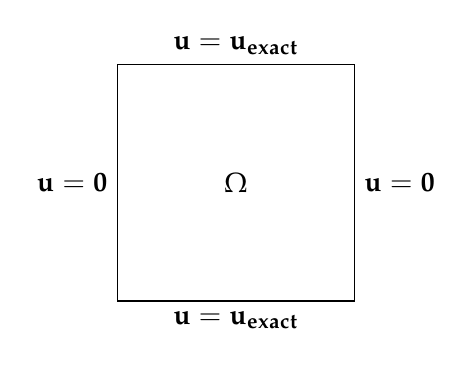
\begin{tikzpicture}
\node[
      draw,
      minimum height=3cm,
      minimum width=3cm,
      label=0:$\mathbf{u=0}$,%< -- This uses angle zero degree on the border for the location
      label=west:$\mathbf{u=0}$, %< -- This uses an anchor of the node for the location
      label=north:$\mathbf{u=u_{exact}}$,
      label=south:$\mathbf{u=u_{exact}}$
] at (0,1.5) {$\Omega$};
\end{tikzpicture}
\end{center}

Let $\mathbf{u}_h$ and $p_h$ be two two approximate solutions obtained from the simulation, we now want compute the errors

\begin{itemize}
\item $|| \mathbf{u}_{exact} - \mathbf{u}_h ||_{L^2}$,
\item $ | \mathbf{u}_{exact} - \mathbf{u}_h |_{H^1}$ (seminorm),
\item $|| p_{exact} - p_h ||_{L^2} $.
\end{itemize}

in order to compare our exact solution with the manufactured one.
Using the previous exact solution, the error is 0, since the method for solving the problem is exact for polynomials, as shown below


\begin{center}
\begin{tabular}{| c | c | c | c |}
\hline
$\mathbf{N}$ & $\mathbf{|| u_{exact} - u_h ||_{L^2}}$ & $ \mathbf{ | u_{exact} - u_h |_{H^1}}$ & $  \mathbf{ || p_{exact} - p_h ||_{L^2}}$ \\
\hline
$ 4 $ & $2.7373 \times 10^{-14}$ & $3.2162 \times 10^{-13}$ &  $ 2.7373 \times 10^{-14}$ \\
\hline
$ 8$ & $1.3173  \times 10^{-12}$ & $7.5841 \times 10^{-11}$ &  $ 1.3172  \times 10^{-12}$ \\
\hline
$ 16 $ & $ 8.4791 \times 10^{-14}$ & $9.1285 \times 10^{-12}$ & $ 8.4791 \times 10^{-14}$ \\
\hline
$ 32$ & $9.0508 \times 10^{-14}$ & $1.6039 \times 10^{-11}$ &  $ 9.0580 \times 10^{-14}$ \\
\hline
$ 64$ & $6.3504 \times 10^{-13}$ & $9.5275 \times 10^{-11}$ &  $ 6.3504 \times 10^{-13}$ \\
\hline
\end{tabular}
\end{center}

\vspace{1cm}

A difference exact solution that could be used is:

\[
\mathbf{u}_{exact} = \left[ \begin{array}{c} 0 \\ sin(\pi x) \end{array} \right], \quad
p_{exact} = \frac{1}{2}-y.
\]

%(Reminder: I put the $\pi$ in order for the exact solution to satisfy the boundary conditions!)
In the following tables, the convergence rate $k$ was computed, according to:

\[
k = \frac{log(\frac{E_{i+1}}{E_i})}{log(\frac{h_{i+1}}{h_i})}
\]

where we are assuming that $E_i \sim h^k_i$ and $E_{i+1} \sim h^k_{i+1}$. \\
The following table shows a second order convergence rate in $H^1$, as confirmed by the convergence plot.

\vspace{1cm}
\begin{figure}[h!]
\centering
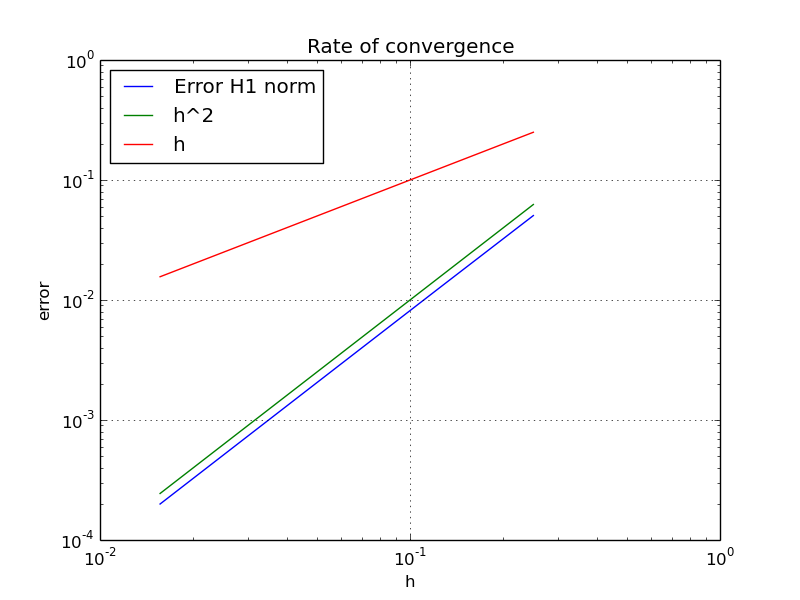
\includegraphics[width=\textwidth]{images/convergence_sine}
\caption{The plot shows a second order convergence, since the blue and green lines are parallel.}
\end{figure}
\vspace{1cm}

\begin{center}
\begin{tabular}{| c | c | c | c | c |}
\hline
$  \mathbf{N}$ & $ \mathbf{|| u_{exact} - u_h ||_{L^2}}$ & $  \mathbf{ | u_{exact} - u_h |_{H^1}}$ & \textbf{Rate in }  $ \mathbf{L^2}$ & \textbf{Rate in } $  \mathbf{H^1}$  \\
\hline
$ 4 $ & $1.9388 \times 10^{-3}$ & $5.0548 \times 10^{-2}$  & & \\
\hline
$ 8$ & $2.4515  \times 10^{-4}$ & $1.2733 \times 10^{-2}$ &  $2.9834$ &  $1.9890$   \\
\hline
$ 16 $ & $ 3.0745 \times 10^{-5}$ & $3.1896 \times 10^{-3}$ & $ 2.9952 $ & $1.9971$   \\
\hline
$ 32$ & $3.8465 \times 10^{-6}$ & $7.9780 \times 10^{-4}$ & $ 2.9987 $ & $ 1.9992 $  \\
\hline
$ 64$ & $4.8092 \times 10^{-7}$ & $1.9948 \times 10^{-4}$  & $ 2.9997 $ & $1.9998$ \\
\hline
\end{tabular}
\end{center}



\begin{center}
\begin{tabular}{| c | c | c |}
\hline
$\mathbf{N}$ & $\mathbf{|| p_{exact} - p_h ||_{L^2}}$ & \textbf{Rate in } $  \mathbf{L^2}$  \\
\hline
$ 4 $ & $1.4420  \times 10^{-4} $ & \\
\hline
$ 8 $ & $ 1.1896  \times 10^{-5} $ & $3.5995$ \\
\hline
$ 16 $ & $ 1.0089  \times 10^{-6} $ & $3.5596$ \\
\hline
$ 32 $ & $  8.7143 \times 10^{-8} $ & $3.5332$ \\
\hline
$ 64 $ & $ 8.0070 \times 10^{-9} $ & $3.4440$ \\
\hline
\end{tabular}
\end{center}


\subsection{MMS for Navier-Stokes equations with parabolic inlet velocity}
\label{parabolic inlet}
We now want to verify our Navier-Stokes solver using MMS. We start from Navier-Stokes equations written in the form (\ref{eq:ns:3}), with $\mu = 1/8$.  Let $\Omega$ be the unit square $\Omega = [0,1]^2$. We want to solve the N-S equation in the domain $\Omega$ applying the following boundary conditions:

\begin{center}
\begin{tikzpicture}
\node[
      draw,
      minimum height=3cm,
      minimum width=3cm,
      label=0:$\sigma \cdot \mathbf{n}$ \text{=}$ -p_{out} \mathbf{n}$,%< -- This uses angle zero degree on the border for the location
      label=west:$\sigma \cdot \mathbf{n}$ \text{=}$ -p_{in} \mathbf{n}$, %< -- This uses an anchor of the node for the location
      label=north:$\mathbf{u=0}$,
      label=south:$\mathbf{u=0}$
] at (0,1.5) {$\Omega$};
\end{tikzpicture}
\end{center}

i.e. $\mathbf{u=0}$ on the top and bottom boundaries, and we apply a pressure difference on the sides, so the fluid can move from left to right. The exact solution for this problem is $\mathbf{u}(y) = [\frac{1}{2\mu} y (1-y), 0]$ and $p(x) = 1-x$. Comparing the numerical solution from our solver with the exact solution, the error is 0:

\begin{center}
\begin{tabular}{| c | c | c | c | c |}
\hline
$\mathbf{N}$ & $\mathbf{dt (= \frac{1}{N})}$ & $\mathbf{|| u_{exact} - u_h ||_{L^2}}$ & $ \mathbf{ | u_{exact} - u_h |_{H^1}}$ & $  \mathbf{ || p_{exact} - p_h ||_{L^2}}$ \\
\hline
$ 4 $ & $ 0.25 $ & $2.5488 \times 10^{-10}$ & $8.0081 \times 10^{-10}$ &  $ 3.7574 \times 10^{-13}$ \\
\hline
$ 8$ & $ 0.125 $ & $6.8121  \times 10^{-11}$ & $2.1401 \times 10^{-10}$ &  $ 1.3412  \times 10^{-14}$ \\
\hline
$ 16 $ & $ 0.0625 $ & $ 3.1065 \times 10^{-11}$ & $9.7595 \times 10^{-11}$ & $ 9.0360 \times 10^{-15}$ \\
\hline
$ 32$ & $ 0.03125 $ & $1.6841 \times 10^{-11}$ & $5.2914 \times 10^{-11}$ &  $ 1.5517 \times 10^{-14}$ \\
\hline
$ 64$ & $ 0.015625 $ & $1.2541 \times 10^{-12}$ & $1.6649 \times 10^{-11}$ &  $ 3.5736 \times 10^{-13}$ \\
\hline
\end{tabular}
\end{center}

\begin{figure}[ht]
\centering
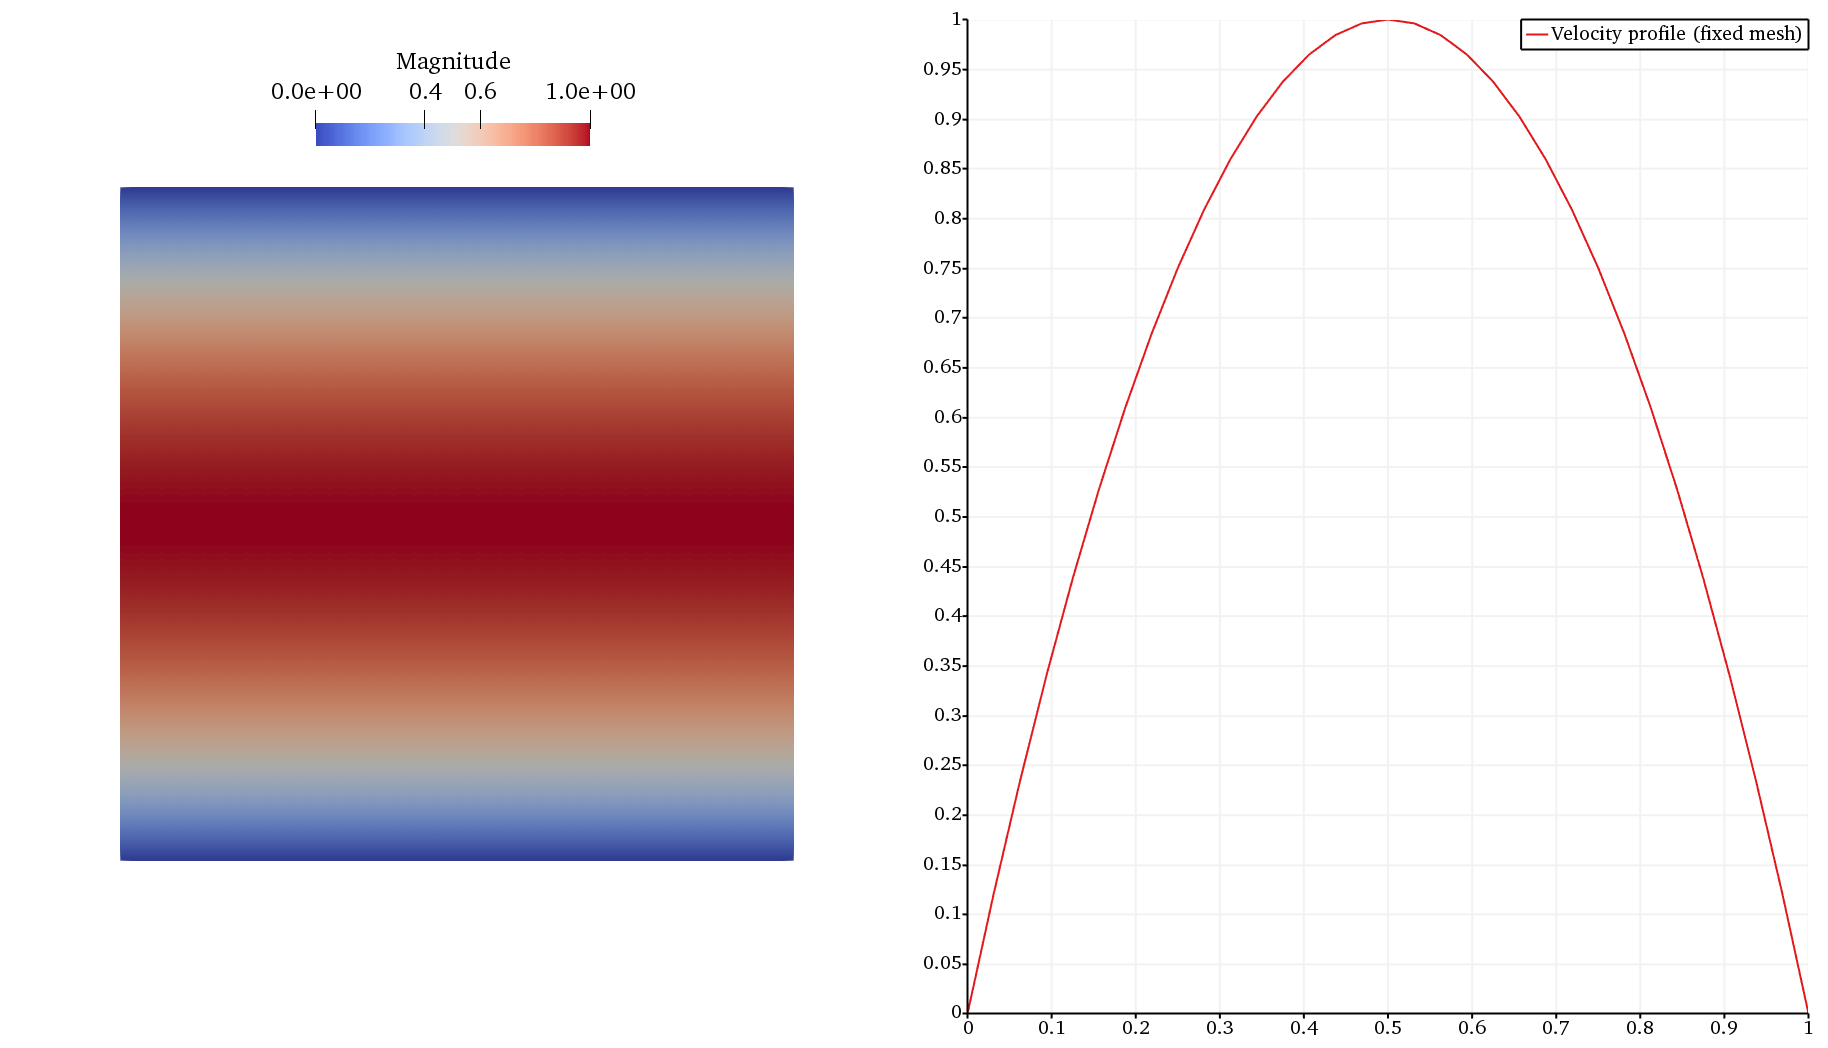
\includegraphics[width=\textwidth]{images/velocity_fixed.png}
\caption{caption}
\end{figure}

\subsection{Pressure-driven channel flow (2D)}
% References:
% Fenics book
% http://faculty.kfupm.edu.sa/CHE/usamah/CHE204/CHE204-HD22%20-%20Flow%20Through%20Circular%20Pipe.pdf

% Should I add some theory on this?

A typical test problem is finding the solution of the Navier-Stokes equations in a two-dimensional pressure-driven channel. We consider a viscous flow between parallel plates, where the geometry is the unit square $[0,1]^2$, and the kinematic viscosity is $\nu = 1/8$. We assume that both plates are fixed, i.e. no-slip boundary conditions are applied to the velocity at the upper and lower walls, and Neumann boundary conditions $\sigma \cdot \vec{n} = 0$ are applied at the inlet and outlet. Dirichlet boundary conditions are applied to the pressure at the inlet and outlet, with $p = 1$ at the inlet and $p = 0$ at the outlet. The initial condition for the velocity is $\mathbf{u} = (0,0)$. As a reference value in order to verify the agreement of our solution, we use the $x$-component of the velocity at the point $(x, y) = (1, 0.5)$ at final time $T = 0.5 $. The value reported on the FEniCS book \cite{logg} is $u_x(1, 0.5, T=0.5) \approx 0.44321183655681595$, while the one obtained in our results is $0.443217320106$.

\begin{figure}[h!]
\centering
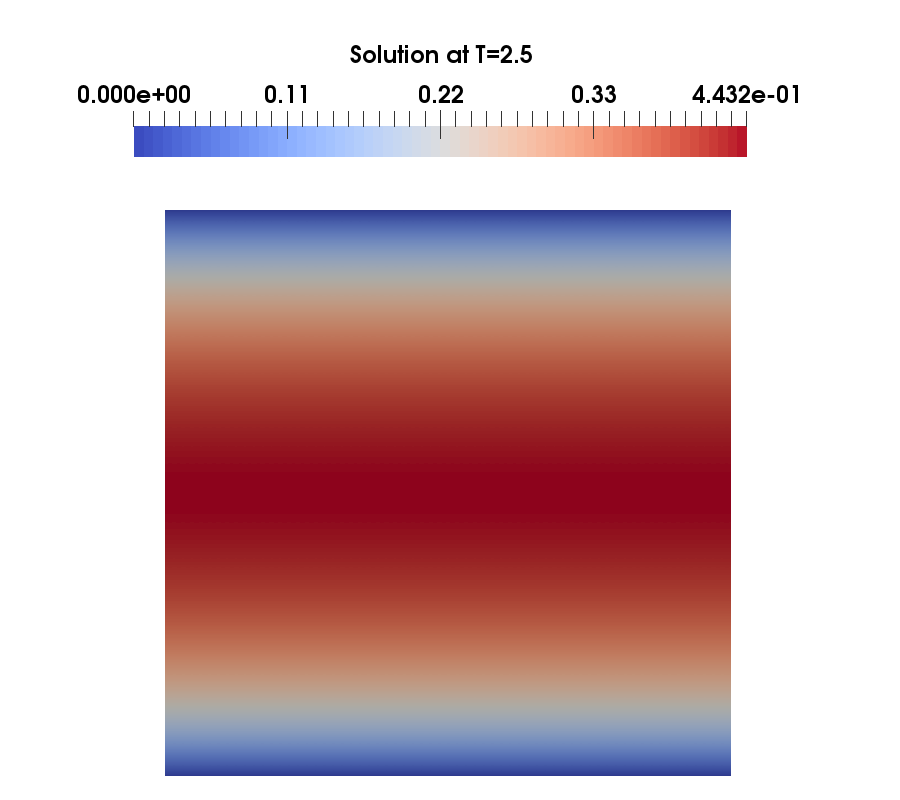
\includegraphics[width=0.8\textwidth]{images/velocity_solution.png}
\caption{Pressure driven channel flow. The plot shows the solution $u(x,y)$ for $\nu = 1/8$.}
\end{figure}

\begin{figure}[h!]
\centering
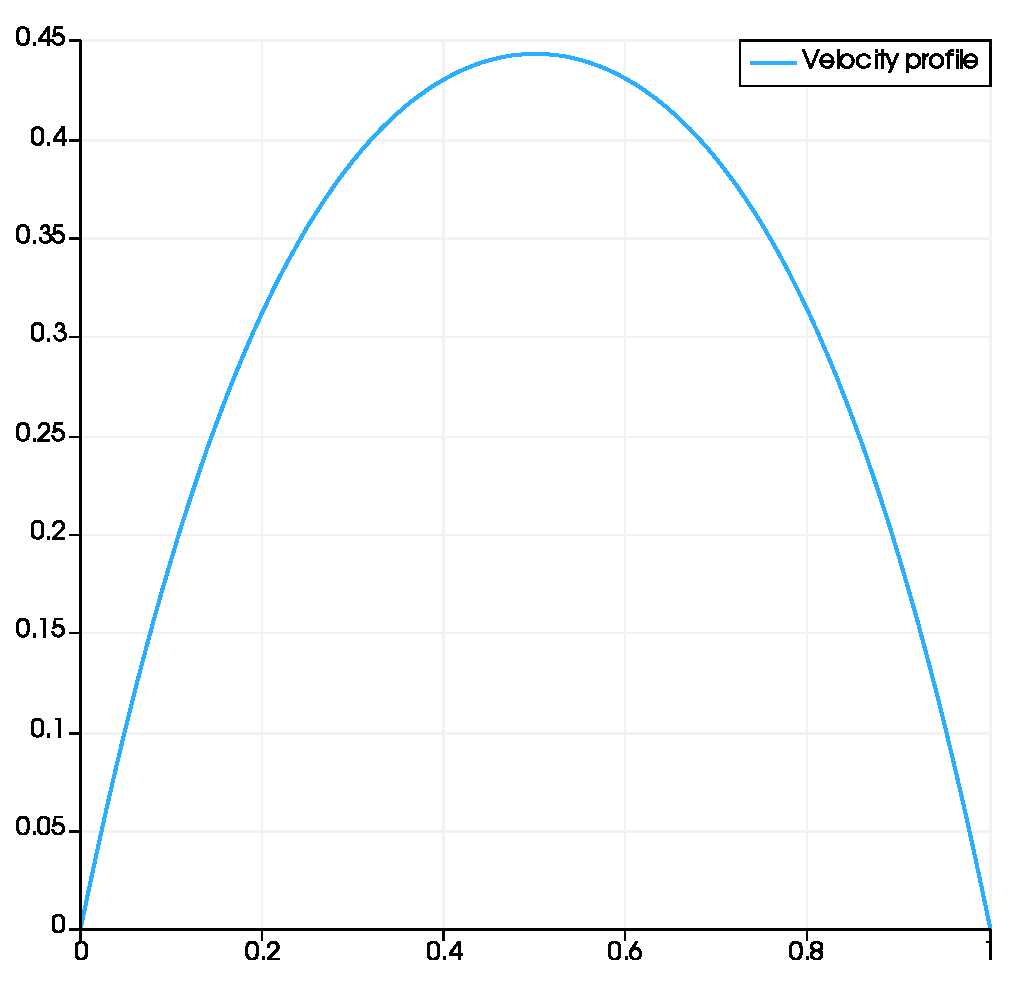
\includegraphics[width=0.6\textwidth]{images/velocity_profile.pdf}
\caption{Pressure driven channel flow. Velocity profile at the points $(0.5, 1)$ and $(0.5, 0)$.}
\end{figure}

\subsection{Driven cavity}
% References:
% Fenics book, Quarteroni, Fluid dynamics F. White

A typical benchmark problem for fluid flow solvers in the two-dimensional lid-driven cavity problem. We consider a square cavity $\Omega$ with sides of unit length, i.e. $\Omega = [0,1] \times [0,1]$, kinematic viscosity $\nu = 1/1000$, and density $\rho = 1$. No-slip boundary conditions are imposed on each edge of the square, except at the upper edge where the velocity is set to $\mathbf{u} = (1,0)^T$, as follows

\[
\begin{cases}
\mathbf{u} = (0, 0)^T, & \mbox{on } \partial \Omega \backslash \Gamma \\
\mathbf{u} = (1, 0)^T, & \mbox{on } \Gamma
\end{cases}
\]

where $ \Gamma = \set{ \mathbf{x} = (x,y)^T \in \partial \Omega | y = 1}$. We use finite elements on triangular grids of the type $\mathcal{P}_2-\mathcal{P}_1$. The initial condition for the velocity is set to zero. The resulting flow is a vortex developing in the upper right corner and then traveling towards the center of the square as the flow evolves. \\
To verify the correctness of the solver, we consider the minimum of the \textit{stream function}. The stream function $\psi$ allows us to satisfy the continuity equation and then solve the momentum equation directly for the single variable $\psi$. It is defined by

\[
\mathbf{u} = \nabla \times \psi = (\frac{\partial \psi}{\partial y} , - \frac{\partial \psi }{\partial x}),
\]

and it can be computed by solving the Poisson problem

\[
- \nabla^2 \psi = \omega,
\]

where $\omega$ is the vorticity given by

\[
\omega = \nabla \times \mathbf{u} = \frac{\partial u_y}{\partial x} - \frac{\partial u_x}{\partial y}.
\]


As a reference value, we use the one reported on the FEniCS book \cite{logg}, where the solution at the final time $T = 2.5$ was computed using the spectral element code Semtex with up to $80 \times 80$ $10^{th}$ order elements, heavily refined in the area in the vicinity of the minimum of the stream function. The time-stepping for computing the reference solution was handled by a third order implicit discretization, and a very short time step was used to minimize temporal errors.  The obtained reference value was $min(\psi) = -0.061 077$.

\begin{figure}[h!]
\centering
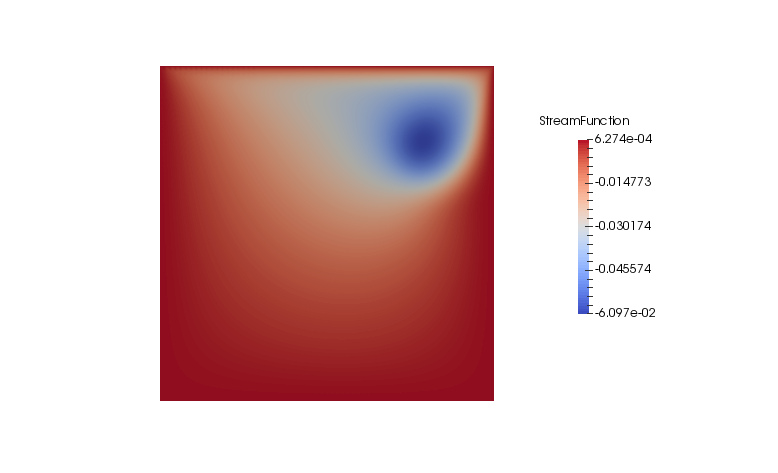
\includegraphics[width=\textwidth]{images/oyvind.png}
\vspace{-1cm}
\caption{Driven cavity. The plot shows the stream function, and its minimum value $-0.06097$. This reference solution is taken from an already validated code \cite{mortensen}.}
\end{figure}


In our case, a Crank-Nicolson (second order) discretization was used, with $\theta = 0.5$. A $64 \times 64$ number of elements was used, with $dt = 0.0125$ as time step. Hence, the obtained value was $min(\psi) = -0.061 121$, in fair agreement with the reference one. \\

\vspace{-.3cm}
\begin{figure}[h!]
\centering
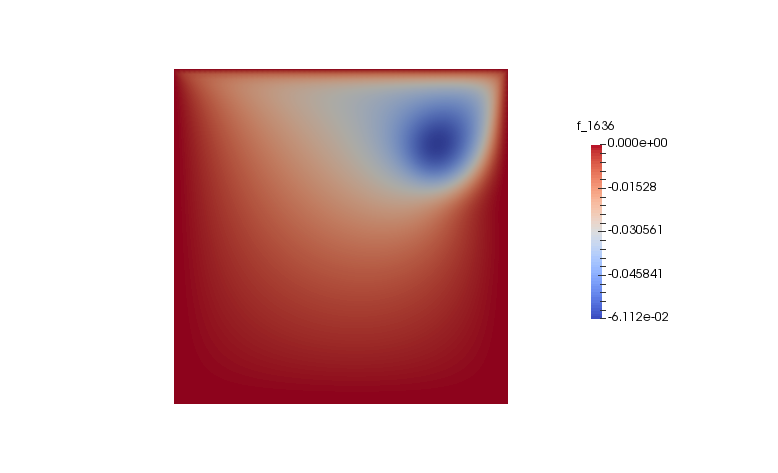
\includegraphics[width=\textwidth]{images/mine.png}
\vspace{-1cm}
\caption{Driven cavity. The plot shows the stream function, and its minimum value $-0.061 121$.}
\end{figure}

%
%\subsection{Nitsche's method}
%Now we want to use the Nitsche method to the driven cavity test case, in order to apply Dirichlet boundary conditions in a weak way. We consider a square cavity $\Omega$ with sides of unit length, i.e. $\Omega = [0,1] \times [0,1]$, kinematic viscosity $\nu = 1/1000$, and density $\rho = 1$. No-slip boundary conditions are imposed on left and bottom edges of the square, except at the upper edge where the velocity is set to $\mathbf{u} = (1,0)^T$, as follows
%
%\[
%\begin{cases}
%\mathbf{u} = (0, 0)^T, & \mbox{on } \partial \Omega \backslash (\Gamma_1 \cup \Gamma_2) \\
%\mathbf{u} = (1, 0)^T, & \mbox{on } \Gamma_1
%\end{cases}
%\]
%
%where $ \Gamma_1 = \set{ (x,y)^T \in \partial \Omega | y = 1}$ and
%$ \Gamma_2 = \set{ (x,y)^T \in \partial \Omega | x = 1}$. On the boundary $\Gamma_2$ we will apply the condition $\mathbf{u} = \mathbf{g} = (0,0)^T$ in a weakly way using Nitsche's method. Substituting (\ref{eq:green}) in (\ref{eq:ns:9}) we have
%
%\begin{align}
%\int_{\Omega} \rho \dot{\mathbf{u}} \, \mathbf{v} \, dx
%+ \int_{\Omega} \rho \nabla \mathbf{u} \cdot (\mathbf{u} - \mathbf{w}) \, \mathbf{v} \, dx
%+ \int_{\Omega} (\mu \nabla \mathbf{u} - pI) \cdot \nabla \mathbf{v} \, dx \\
%- \int_{\partial \Omega} (\mu \nabla \mathbf{u} - pI) \cdot \mathbf{n} \, \mathbf{v} \, ds.
%= \int_{\Omega} \mathbf{f} \mathbf{v} \, dx.
%\end{align}
%
%Since we are applying Dirichlet boundary conditions on $\partial \Omega \backslash \Gamma_2$, $\mathbf{v} = (0,0)$, hence 
%
%\begin{align}
%\int_{\Omega} \rho \dot{\mathbf{u}} \, \mathbf{v} \, dx
%+ \int_{\Omega} \rho \nabla \mathbf{u} \cdot (\mathbf{u} - \mathbf{w}) \, \mathbf{v} \, dx
%+ \int_{\Omega} (\mu \nabla \mathbf{u} - pI) \cdot \nabla \mathbf{v} \, dx \\
%- \int_{\Gamma_2} (\mu \nabla \mathbf{u} - pI) \cdot \mathbf{n} \, \mathbf{v} \, ds.
%= \int_{\Omega} \mathbf{f} \mathbf{v} \, dx.
%\end{align}
%
%and from (\ref{eq:bc:5}), the latter can be written as
%
%\begin{align}
%\int_{\Omega} \rho \dot{\mathbf{u}} \, \mathbf{v} \, dx
%+ \int_{\Omega} \rho \nabla \mathbf{u} \cdot (\mathbf{u} - \mathbf{w}) \, \mathbf{v} \, dx
%+ \int_{\Omega} (\mu \nabla \mathbf{u} - pI) \cdot \nabla \mathbf{v} \, dx \\
%- \int_{\Gamma_2} (\mu \frac{\partial \mathbf{u}}{\partial \mathbf{n}} -  p \mathbf{n}) \, \mathbf{v} \, ds
%= \int_{\Omega} \mathbf{f} \mathbf{v} \, dx.
%\end{align}
%
%We now apply the Nitsche method on the boundary term $\Gamma_2$, that leads to
%
%\begin{align}
%\int_{\Omega} \rho \dot{\mathbf{u}} \, \mathbf{v} \, dx
%+ \int_{\Omega} \rho \nabla \mathbf{u} \cdot (\mathbf{u} - \mathbf{w}) \, \mathbf{v} \, dx
%+ \int_{\Omega} (\mu \nabla \mathbf{u} - pI) \cdot \nabla \mathbf{v} \, dx \\
%- \int_{\Gamma_2} \mu \frac{\partial \mathbf{u}}{\partial \mathbf{n}} \, \mathbf{v} \, ds
%- \int_{\Gamma_2} \mu \frac{\partial \mathbf{v}}{\partial \mathbf{n}}  \, \mathbf{u} \, ds
%+ \frac{\gamma}{h} \int_{\Gamma_2} \mathbf{u \, v} ds \\
%= - \int_{\Gamma_2} \mu \frac{\partial \mathbf{v}}{\partial \mathbf{n}}  \, \mathbf{g} \, ds
%+ \frac{\gamma}{h} \int_{\Gamma_2} \mathbf{g \, v} ds
%+  \int_{\Omega} \mathbf{f} \mathbf{v} \, dx.
%\end{align}
%
%A $128 \times 128$ number of elements was used with $dt = 0.0125$ as time step. The obtained value was $min(\psi) = -0.0597826179273$. 
%
%\begin{figure}[ht]
%\centering
%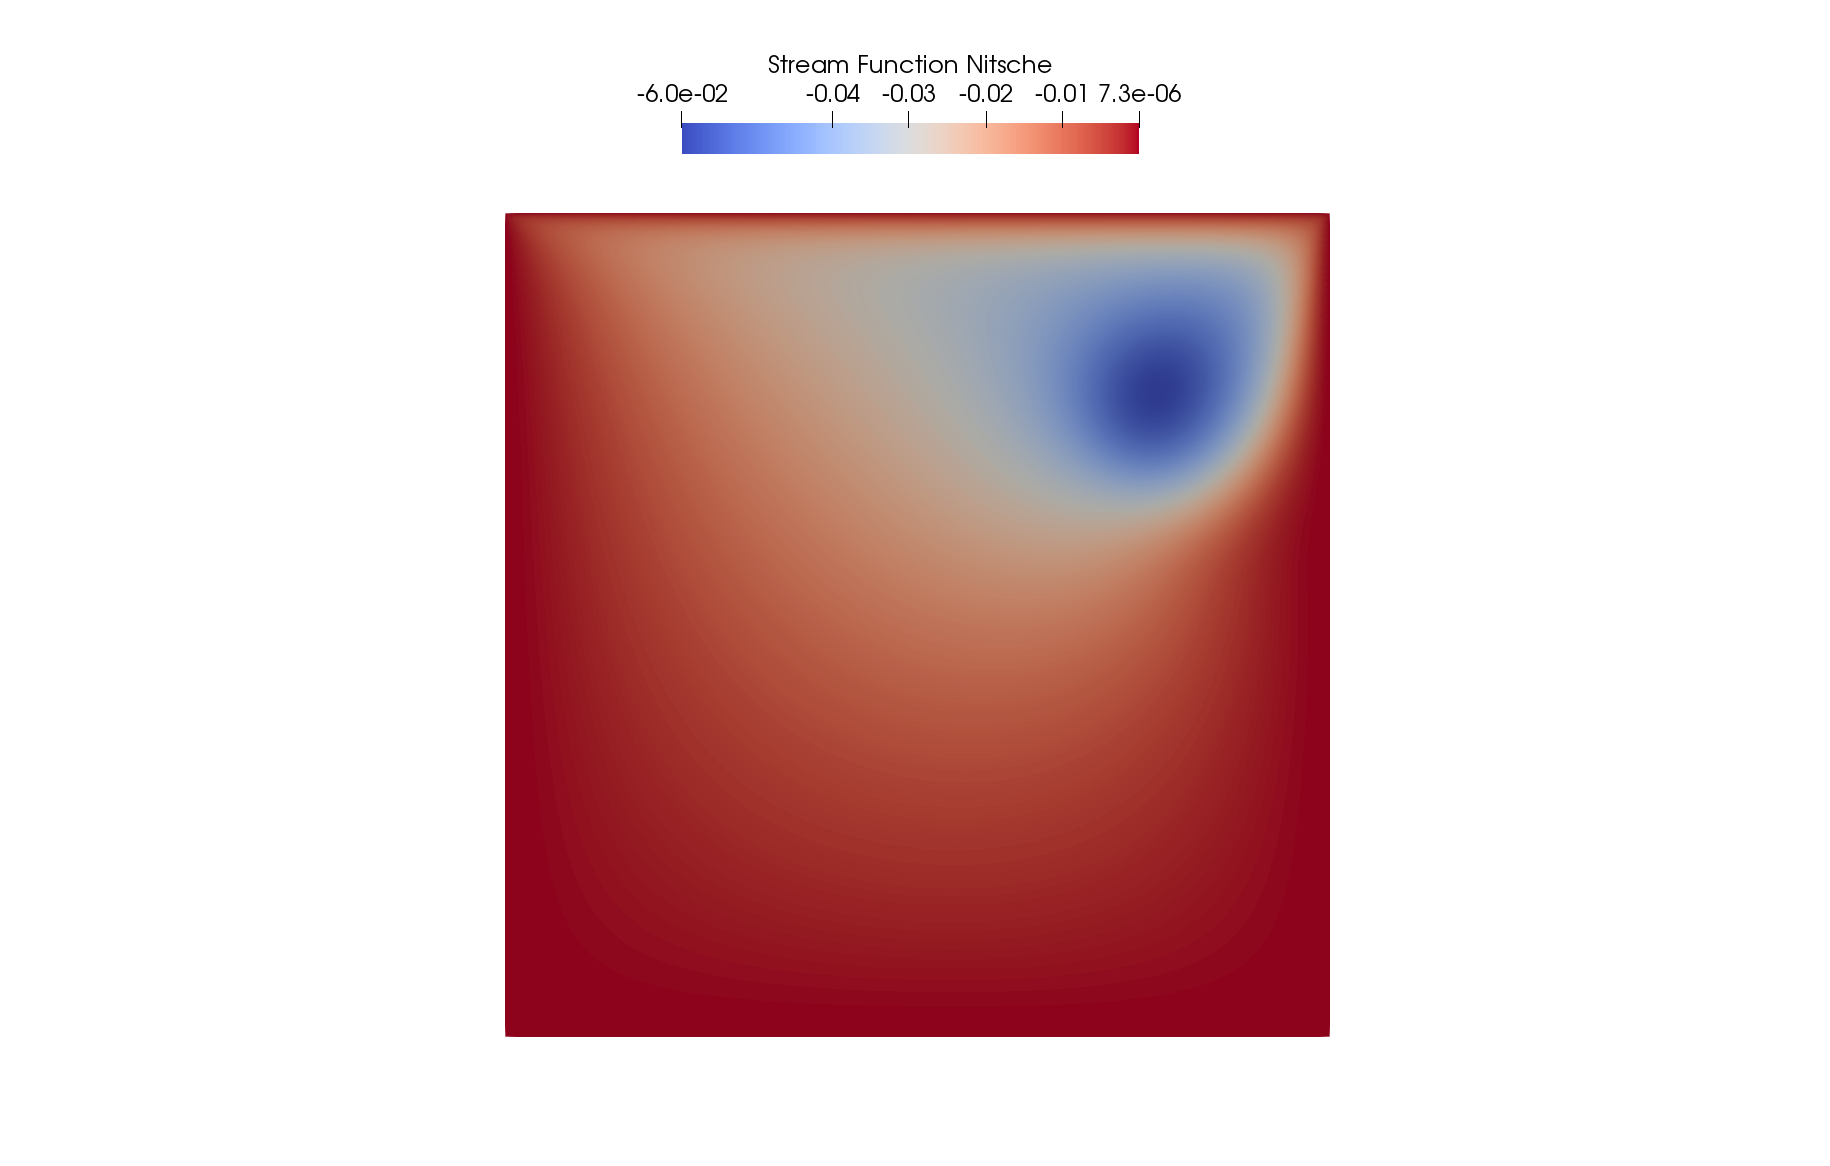
\includegraphics[width=\textwidth]{images/stream_function_nitsche.png}
%\vspace{-1cm}
%\caption{Driven cavity with Nitsche. The plot shows the stream function, and its minimum value $-0.05978$.}
%\end{figure}

\newpage

\section{Navier-Stokes equations on a moving mesh}
\subsection{Parabolic inlet velocity with fixed mesh motion}
In this section we add a fixed mesh motion to the test case in section \ref{parabolic inlet}. We start from the NS equations with ALE term written in the form (\ref{eq:ns:1})-(\ref{eq:ns:2}) with $\mu = 1/8$. In our case, the rigid motion will be given by the vector $\mathbf{w} = [0.05, 0.05]^T$. The solution is qualitatively the same as in section \ref{parabolic inlet}, as shown by the following plot, where we plotted the velocity profile between the points $(0.5, 0)$ and $(0.5, 1)$.

\begin{figure}[h!]
\centering
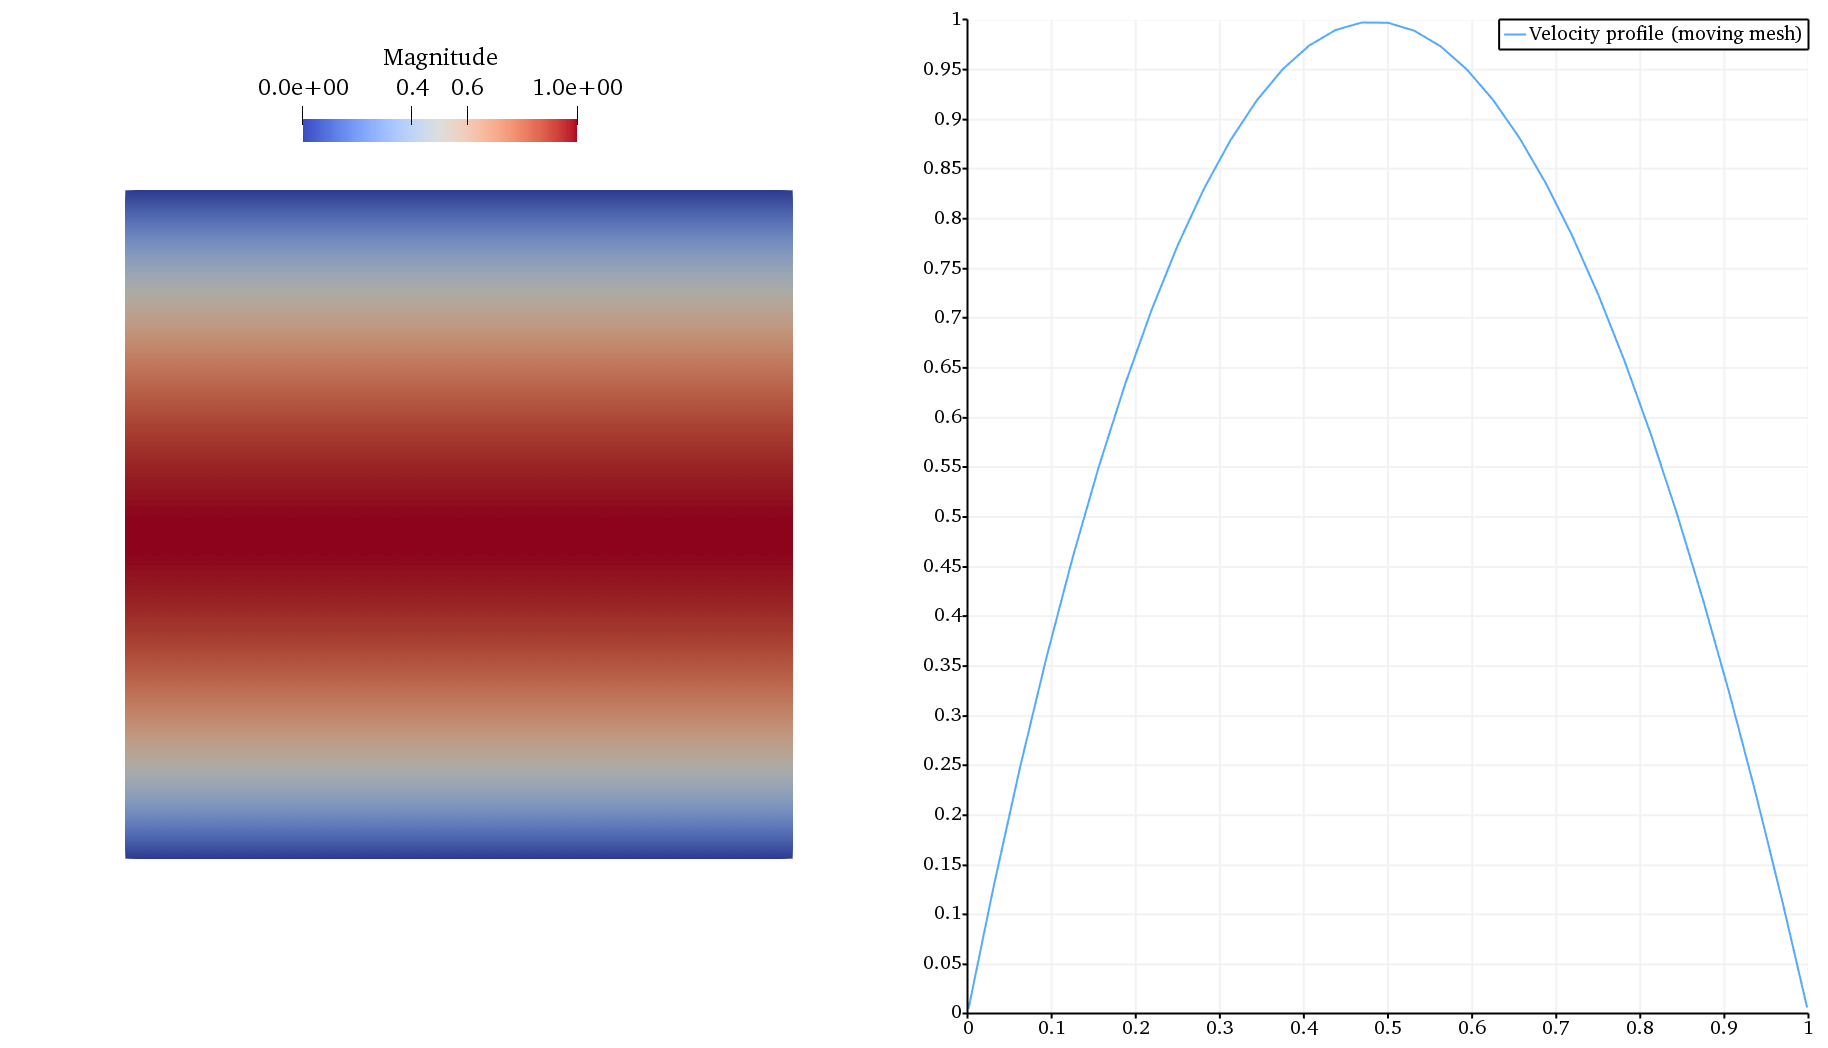
\includegraphics[width=\textwidth]{images/velocity_moving.png}
\caption{caption}
\end{figure}

\chapter{SAS simulations}

\section{Mesh refinement on the fixed mesh}
The first step is to ensure that our solution to the Navier-Stokes equations that we solved numerically is grid independent. To this purpose, we did a mesh refinement test on the rectangular mesh, which consists of $N$ elements on shorter boundaries (top and bottom), and $10 \cdot N$ element on the longer one (cord and tissue). We then plotted the $x$ component of the velocity field $\mathbf{v}$ in the point $(x,y) = (2, 60)$ and compared it for different values of $N$. The time step is $\Delta t = 0.00625$. 

\begin{figure}[h!]

\centering
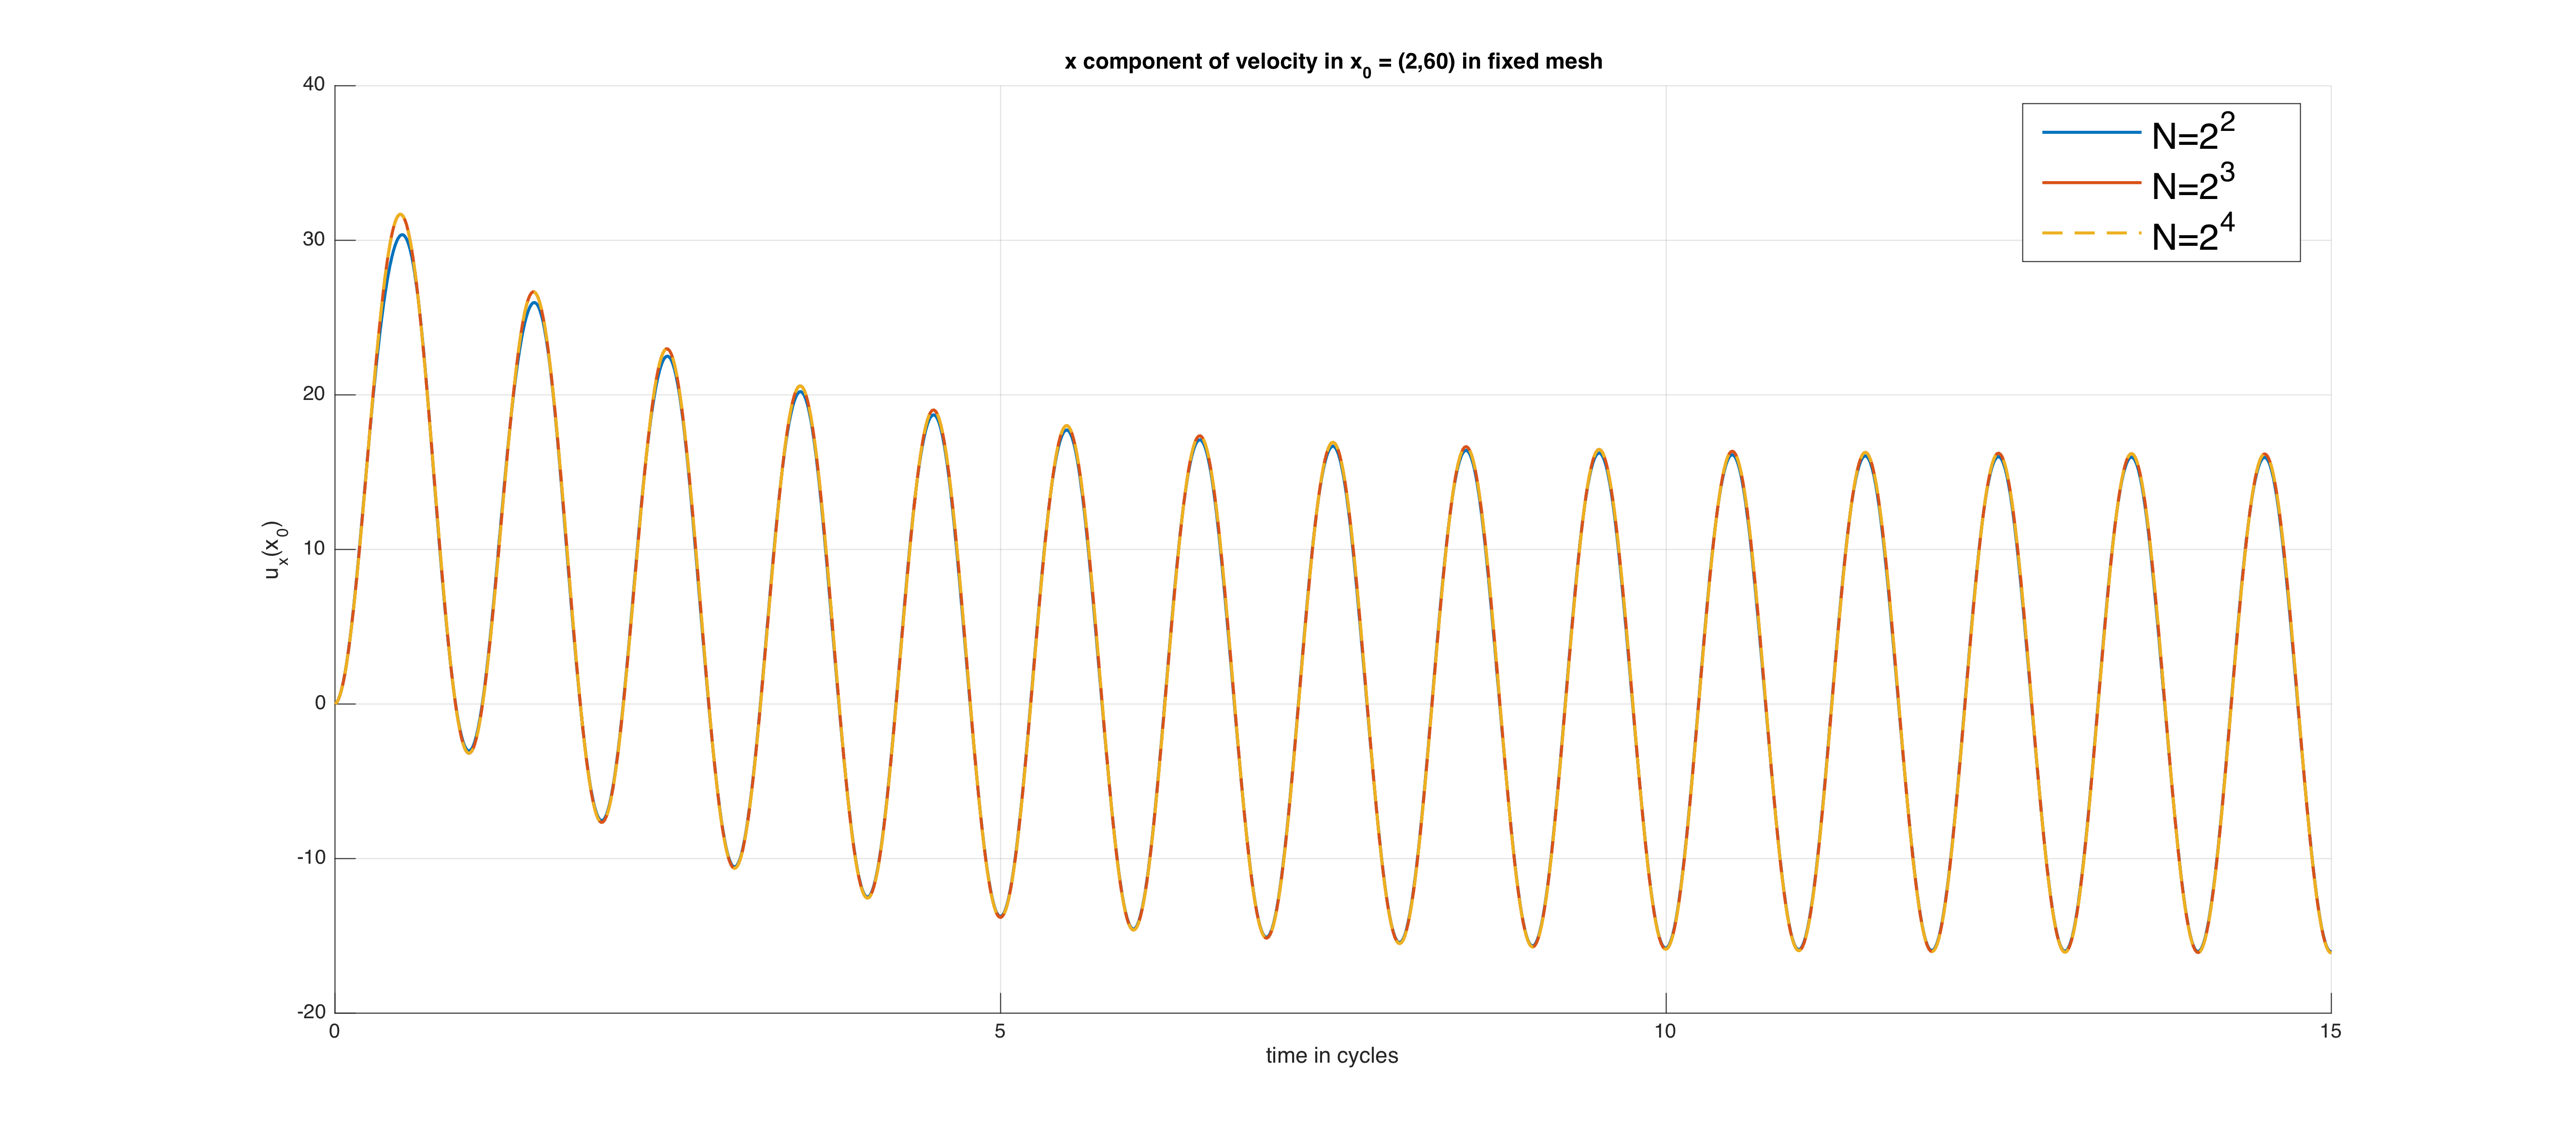
\includegraphics[width=\textwidth]{images/mesh_refinement}
\caption{Plot of the $x$ component of the velocity field in the point $(x,y)=(2,60)$.}
\label{img:sas:1}
\end{figure}

From the mesh refinement study we decided to use $N=2^3$ for the further simulations since it is a good compromise between accuracy and computational cost.
We can see that the flow needs several cycles to fully develop, and that is why in the future simulations we will focus only on the last cycle.


\section{Comparison between fixed and moving meshes}
We now want to compare different quantities between the fixed and the moving meshes.  CITE \cite{elliott}  \cite{hung} \cite{bertram} SOMEWHERE



\chapter{Conclusions}


\begin{thebibliography}{100}
\addcontentsline{toc}{chapter}{Bibliography}

\bibitem{alperin1} N. Alperin, J. R. Loftus, A. M. Bagci, S. H. Lee, C. J. Oliu, A. H. Shah, B. A. Green, \emph{Magnetic resonance imaging- based methods measures predictive of short-term surgical outcome in patients with Chiari malformation Type I: a pilot study}, J. Neurosurg. Spine, 2016.

\bibitem{alperin2} N. J. Alperin, S. H. Lee, F. Loth, P. B. Raksin, T. Lichtor, \emph{MR-Intracranial Pressure (ICP): a method to measure intracranial elastance and pressure noninvasively by means of MR imaging: baboon and humany study}, Radiology, 2000.

\bibitem{barth} W. L. Barth and G. F. Carey, \emph{On a boundary condition for pressure-driven laminar flow of incompressible fluids}, International journal for numerical methods in fluids, vol. 54, no. 11, pp. 1313–1325, 2007.


\bibitem{bejjani} G. K. Bejjani, \emph{Definition of the adult Chiari malformation: a brief historical overview}, Neurosurg Focus, 2001; 11(1).

\bibitem{bertram} C. Bertram, L. Bilston, and M. Stoodley, \emph{Tensile radial stress in the spinal cord related to arachnoiditis or tethering: a numerical model}, Medical \& Biological engineering \& Computing, vol. 46, no. 7, pp. 701-707, 2008.

\bibitem{brenner} S. Brenner and R. Scott, \emph{The mathematical theory of finite element methods}, vol. 15. Springer Science \& Business Media, 2007.

\bibitem{clarke} E. C. Clarke, D. F. Fletcher, M. A. Stoodley, and L. E. Bilston, \emph{Computational fluid dynamics modelling of cerebrospinal fluid pressure in Chiari malformation and syringomyelia}, Journal of biomechanics, vol. 46, no. 11, pp. 1801–1809,
2013.

\bibitem{dolar} M. T. Dolar, V. M. Haughton, B. J. Iskandar, M. Quigley, \emph{Effect of Craniocervical Decompression on peak CSF velocities in symptomatic patients with Chiari I malformation}, AJNR Am. J. Neuroradiol. 25:142-145, 2004.

\bibitem{donea} J. Donea, A. Huerta, J. Ponthot, A. Rodriguez-Ferran, \emph{Arbitrary Lagrangian-Eulerian Methods} Encyclopedia of Computational Mechanics Vol. 1, Wiley \& Sons, 2004.

\bibitem{drosdal} I. N. Drosdal, \emph{Porous and viscous modeling of cerebrospinal fluid flow in the spinal canal associated with syringomyelia}, 2011.

\bibitem{duarte} F. Duarte, R. Gormaz, S. Natesan, \emph{Arbitrary Lagrangian-Eulerian method for Navier-Stokes equations with moving boundaries}, Comput. Methods Appl. Mech. Engrg, 193 (2004) 4819-4836.

\bibitem{elliott} N. Elliott, C. Bertram, B. A. Martin, and A. Brodbelt, \emph{Syringomyelia: A review of the biomechanics}, Journal of Fluids and Structures, vol. 40, pp. 1-24, 2013.


\bibitem{fletcher} T. M. Fletcher, B. Wirthl, A. G. Kolias, H. Adams, P. J. A. Hutchinson, M. P. F. Sutcliffe, \emph{Modelling of brain deformation after decompressive craniectomy}, Annals of Biomedical Engineering, 2016.

\bibitem{goriely} A. Goriely, M. G. D. Geers, G. A. Holzapfel, J. Jayamohan, A. Jérusalem, S. Sivaloganathan, W. Squier, J. A. W. van Dommelen, S. Waters, E. Kuhl., \emph{Mechanics of the brain: perspectives, challenges, and opportunities}, Biomech. Model. Mechanobiol. 14: 931-965, 2015.


\bibitem{greitz} D. Greitz, \emph{Unraveling the riddle of syringomyelia}, Neurosurg. Rev. (2006), 29: 251-264.

\bibitem{haughton1} V. M. Haughton, F. R. Korosec, J. E. Medow, M. T. Dolar, and B. J. Iskan- dar, \emph{Peak systolic and diastolic CSF velocity in the foramen magnum in adult patients with Chiari I malformations and in normal control participants},” American Journal of Neuroradiology, vol. 24, no. 2, pp. 169-176, 2003.

\bibitem{haughton2} V. Haughton and K.-A. Mardal, \emph{Spinal fluid biomechanics and imaging: an update for neuroradiologists}, American Journal of Neuroradiology, vol. 35, no. 10, pp. 1864–1869, 2014.


\bibitem{he} Y. He, W. Sun, \emph{Stability and convergence of the Crank-Nicolson/Adams-Bashforth scheme for the time-dependent Navier-Stokes equations}, SIAM J. Numer. Anal. Vol. 45, No. 2, 837-869.

\bibitem{heiss} J. D. Heiss, G. Suffredini, K. D. Bakhtian, M. Sarntinoranont, E. H. Oldfield, \emph{Normalization of hindbrain morphology after decompression of Chiari malformation Type I}, J. Neurosurg 117:942:946, 2012.


\bibitem{hron} J. Hron, S. Turek, \emph{A monolithic FEM/multigrid solver for an ALE formula- tion of fluid-structure interaction with applications in biomechanics}. Springer, 2006.

\bibitem{hung} T. K. Hung, G. L. Chang, H. S. Lin, F. R. Walter, and L. Bunegin, \emph{Stress- strain relationship of the spinal cord of anesthetized cats}, Journal of biomechanics, vol. 14, no. 4, pp. 269-276, 1981

\bibitem{iskandar} B. J. Iskandar, M. Quigley, V. M. Haughton, \emph{Foramen magnum cerebrospinal fluid flow characteristics in children with Chiari I malformation before and after craniovertebral decompression}, J. Neurosurg. (Pediatrics 2) 101: 169-178, 2004.


\bibitem{linge1}  S. Linge, V. Haughton, A. E. Løvgren, K.-A. Mardal, A. Helgeland, and H. P. Langtangen, \emph{Effect of tonsillar herniation on cyclic CSF flow studied with computational flow analysis}, American Journal of Neuroradiology, vol. 32, no. 8, pp. 1474–1481, 2011.

\bibitem{linge2} S. O. Linge, K.-A. Mardal, A. Helgeland, J. D. Heiss, and V. Haughton, \emph{Effect of craniovertebral decompression on CSF dynamics in chiari malformation type i studied with computational fluid dynamics: Laboratory investigation}, Journal of neurosurgery. Spine, vol. 21, no. 4, p. 559, 2014.

\bibitem{linge3} S. Linge, V. Haughton, A. Løvgren, K. Mardal, and H. Langtangen, \emph{CSF flow dynamics at the craniovertebral junction studied with an idealized model of the subarachnoid space and computational flow analysis}, American Journal of Neuroradiology, vol. 31, no. 1, pp. 185-192, 2010.


\bibitem{logg} A. Logg, K.-A. Mardal, and G. Wells, \emph{Automated solution of differential equations by the finite element method: The FEniCS book}, vol. 84. Springer Science \& Business Media, 2012.


\bibitem{martin1} B. A. Martin and F. Loth, \emph{The influence of coughing on cerebrospinal fluid pressure in an in vitro syringomyelia model with spinal subarachnoid space stenosis}, Cerebrospinal Fluid Res, vol. 6, no. 1, p. 17, 2009.

\bibitem{martin2} B. A. Martin, R. Labuda, T. J. Royston, J. N. Oshinski, B. Iskandar, and F. Loth, \emph{Spinal subarachnoid space pressure measurements in an in vitro spinal stenosis model: implications on syringomyelia theories}, Journal of Biomechanical Engineering, vol. 132, no. 11, p. 111007, 2010.

\bibitem{martin3} B. A. Martin, W. Kalata, F. Loth, T. J. Royston, and J. N. Oshinski, \emph{Sy ringomyelia hydrodynamics: an in vitro study based on in vivo measurements}, Journal of biomechanical engineering, vol. 127, no. 7, pp. 1110-1120, 2005.

\bibitem{martin4} B. A. Martin, R. Labuda, T. J. Royston, J. N. Oshinski, B. Iskandar, and F. Loth, \emph{Pathological biomechanics of cerebrospinal fluid pressure in syringomyelia: Fluid structure interaction of an in vitro coaxial elastic tube system}, pp. 941-942, 2009.

\bibitem{martin5} B. A. Martin, W. Kalata, F. Loth, T. J. Royston, J. N. Oshinski, \emph{Syringomyelia Hydrodynamics: an in vitro study based on in vivo measurements}, Journal of Biomechanical Engineering, vol. 127, December 2005.


\bibitem{mortensen} M. Mortensen, K. Valen-Sendstad, \emph{Oasis: a high-level/high performance open source Navier-Stokes solver}, Computer Physics Communications, Vol. 188, pp. 177-188, 2016.

\bibitem{quarteroni1} A. Quarteroni, A. Valli, \emph{Numerical approximation of partial differential equations}, Springer, 2008.
\bibitem{quarteroni2} A. Quarteroni, \emph{Numerical Models for Differential Problems}, Springer, 2014.

\bibitem{raksin} P. B. Raksin, N. Alperin, A. Sivaramakrishnan, S. Surapaneni, T. Lichtor, \emph{Noninvasive intracranial compliace and pressure based on dynamic magnetic resonance imaging of blood flow and cerebrospinal fluid flow}, Neurosurg. Focus 2003; 14(4).

\bibitem{reynolds} O. Reynolds, \emph{Papers on Mechanical and Physical Subjects, The Sub-Mechanics of the Universe}, vol. 3. Cambridge University Press, Cambridge, 1903.

\bibitem{rutkowska1}  G. Rutkowska, V. Haughton, S. Linge, and K.-A. Mardal, \emph{Patient-specific 3d simulation of cyclic CSF flow at the craniocervical region}, American Journal of Neuroradiology, vol. 33, no. 9, pp. 1756–1762, 2012.

\bibitem{rutkowska2} G. Rutkowska, \emph{Computational fluid dynamics in patient-specific models of normal and Chiari I geometries}, 2011.

\bibitem{silverthorn} D.U. Silverthorn, \emph{Human Physiology}, 7th edition.

\bibitem{sivarama} A. Sivaramakrishnan, N. Alperin, S. Surapaneni, T. Lichtor, \emph{Evaluating the effet of decompression surgery on cerebrospinal fluid flow and intracranial compliance in patients with Chiari malformation with magnetic resonance imaging flow studies}, Neurosurgery, 55:1344-1351, 2004.

\bibitem{stoverud1} K. H. Støverud, M. Alnæs, H. P. Langtangen, V. Haughton, and K.-A. Mardal, \emph{Poro-elastic modeling of syringomyelia–a systematic study of the effects of pia mater, central canal, median fissure, white and gray matter on pressure wave propagation and fluid movement within the cervical spinal cord}, Computer methods in biomechanics and biomedical engineering, pp. 1-13, 2015.

\bibitem{stoverud2} K. H. Stoverud, \emph{Relation between the Chiari I malformation and syringomyelia from a mechanical perspective}, 2014.

\bibitem{taylor} C. Taylor and P. Hood, \emph{A numerical solution of the Navier-Stokes equations using the finite element technique}, Computers \& Fluids, vol. 1, no. 1, pp. 73-100, 1973.

\bibitem{thompson} A. Thompson, N. Madan, J. Hesselink, G. Weinstein, A. M. del Rio, and V. Haughton, \emph{The cervical spinal canal tapers differently in patients with Chiari I with and without syringomyelia}, American Journal of Neuroradiology, 2015.

\bibitem{tremblay} D. Tremblay, S. Etienne, D. Pelletier, \emph{Code verification and the method of manifactured solutions for fluid-structure interaction problems}, 36th AIAA Fluid Dynamics Conference and Exhibit, 2006.

\bibitem{vegard} V. Vinje, \emph{Simulating cerebrospinal fluid flow and spinal cord movement associated with syringomyelia}, 2016.

\bibitem{white} F. M. White, \emph{Fluid mechanics}, 7th edition.


\end{thebibliography}

\end{document}
